%%%%%%%%%%%%%%%%%%%%%%%%%%%%%%%%%%%%%%%%%%%%%%%%%%%%%%%%%%%%%%%%%%%%%%%%
%% Customizações do abnTeX2 (http://abnTeX2.googlecode.com)           %%
%% para a Universidade de Fortaleza						              %%
%%                                                                    %%
%% This work may be distributed and/or modified under the             %%
%% conditions of the LaTeX Project Public License, either version 1.3 %%
%% of this license or (at your option) any later version.             %%
%% The latest version of this license is in                           %%
%%   http://www.latex-project.org/lppl.txt                            %%
%% and version 1.3 or later is part of all distributions of LaTeX     %%
%% version 2005/12/01 or later.                                       %%
%%                                                                    %%
%% This work has the LPPL maintenance status `maintained'.            %%
%%                                                                    %%
%% The Current Maintainer of this work is Bruno Lopes                 %%
%%                                                                    %%
%% Project available on: https://github.com/bruno-unifor/unifortex2   %%
%%                                                                    %%
%% Further information about abnTeX2                                  %%
%% are available on http://abntex2.googlecode.com/                    %%
%%                                                                    %%
%%%%%%%%%%%%%%%%%%%%%%%%%%%%%%%%%%%%%%%%%%%%%%%%%%%%%%%%%%%%%%%%%%%%%%%%

\documentclass[
    a4paper,          % Tamanho da folha A4
    12pt,             % Tamanho da fonte 12pt
    chapter=TITLE,    % Todos os capitulos devem ter caixa alta
    section=TITLE,    % Todas as secoes devem ter caixa alta
    oneside,          % Usada para impressao em apenas uma face do papel
    english,          % Hifenizacoes em ingles
    spanish,          % Hifenizacoes em espanhol
    brazil            % Ultimo idioma eh o idioma padrao do documento
]{abntex2}

% Importações de pacotes
\usepackage[brazil]{babel} 
\usepackage[utf8]{inputenc}                         % Acentuação direta
\usepackage[T1]{fontenc}                            % Codificação da fonte em 8 bits
\usepackage{graphicx}                               % Inserir figuras
\usepackage{amsfonts, amssymb, amsmath}             % Fonte e símbolos matemáticos
\usepackage{booktabs}                               % Comandos para tabelas
\usepackage{verbatim}                               % Texto é interpretado como escrito no documento
\usepackage{multirow, array}                        % Múltiplas linhas e colunas em tabelas
\usepackage{indentfirst}                            % Endenta o primeiro parágrafo de cada seção.
\usepackage{listings}                               % Utilizar codigo fonte no documento
\usepackage{xcolor}
\usepackage{microtype}                              % Para melhorias de justificação?
\usepackage[portuguese,ruled,lined]{algorithm2e}    % Escrever algoritmos
\usepackage{algorithmic}                            % Criar Algoritmos
%\usepackage{float}                                  % Utilizado para criação de floats
\usepackage{amsgen}
\usepackage{lipsum}                                 % Usar a simulação de texto Lorem Ipsum
%\usepackage{titlesec}                               % Permite alterar os títulos do documento
\usepackage{tocloft}                                % Permite alterar a formatação do Sumário
\usepackage{etoolbox}                               % Usado para alterar a fonte da Section no Sumário
\usepackage[nogroupskip,nonumberlist,acronym]{glossaries}                % Permite fazer o glossario
\usepackage{caption}                                % Altera o comportamento da tag caption
\usepackage[alf, abnt-emphasize=bf, bibjustif, recuo=0cm, abnt-etal-cite=3, abnt-etal-list=0,abnt-etal-text=it]{abntex2cite}  % Citações padrão ABNT
%\usepackage[bottom]{footmisc}                      % Mantém as notas de rodapé sempre na mesma posição
%\usepackage{times}                                 % Usa a fonte Times
\usepackage{mathptmx}                               % Usa a fonte Times New Roman
%\usepackage{lmodern}                               % Usa a fonte Latin Modern
%\usepackage{subfig}                                % Posicionamento de figuras
%\usepackage{scalefnt}                              % Permite redimensionar tamanho da fonte
%\usepackage{color, colortbl}                       % Comandos de cores
%\usepackage{lscape}                                % Permite páginas em modo "paisagem"
%\usepackage{ae, aecompl}                           % Fontes de alta qualidade
%\usepackage{picinpar}                              % Dispor imagens em parágrafos
%\usepackage{latexsym}                              % Símbolos matemáticos
%\usepackage{upgreek}                               % Fonte letras gregas
\usepackage{appendix}                               % Gerar o apendice no final do documento
\usepackage{paracol}                                % Criar paragrafos sem identacao
\usepackage{lib/unifortex2}		                    % Biblioteca com as normas da Unifor para trabalhos academicos
\usepackage{pdfpages}                               % Incluir pdf no documento
\usepackage{amsmath}                                % Usar equacoes matematicas
 
 % Organiza e gera a lista de abreviaturas, simbolos e glossario
\makeglossaries
 
 % Usar Euro
\usepackage{eurosym}
 % Usar landscape mode
\usepackage{lscape}

% Gera o Indice do documento
\makeindex

%figura+
\usepackage{subcaption}
\usepackage{float}


\trabalhoacademico{tccgraduacao}

\removerbordasdohyperlink{sim}

\cordohyperlink{nao}

\ies{Universidade de Fortaleza}
\iessigla{UNIFOR}
\centro{Centro de Ciências Tecnológicas}

\graduacaoem{Ciência da Computação}
\habilitacao{bacharel}

\autor{NICHOLAS MESQUITA CABRAL DOS ANJOS}
\titulo{Análise de desempenho de algoritmos de compressão de imagens em ambientes hospitalares}
\data{2024}
\local{Fortaleza -- Ceará}

\dataaprovacao{01 de Dezembro de 2020}

\orientador{Prof. Dr. Napoleão Vieira Nepomuceno}
\orientadories{Universidade de Fortaleza - UNIFOR}
\orientadorcentro{Centro de Ciências Tecnológicas - CCT}
\orientadorfeminino{nao} % Coloque 'sim' se for do sexo feminino

\coorientador{}
\coorientadories{Universidade Co-orientador - SIGLA}
\coorientadorcentro{Centro do Co-orientador - SIGLA}
\coorientadorfeminino{nao} % Coloque 'sim' se for do sexo feminino

\membrodabancadois{Membro da Banca Dois}
\membrodabancadoiscentro{Centro de Ciências e Tecnologia - CCT}
\membrodabancadoisies{Universidade do Membro da Banca Dois - SIGLA}

\membrodabancatres{Membro da Banca Três}
\membrodabancatrescentro{Centro de Ciências e Tecnologia - CCT}
\membrodabancatresies{Universidade do Membro da Banca Três - SIGLA}

% \usepackage{graphicx}
% \usepackage{algorithm}
% \usepackage{algpseudocode}
% \usepackage[linesnumbered,ruled,vlined]{algorithm2e}
% \graphicspath{{./images/}}
% \usepackage[breaklinks=true]{hyperref}
\usepackage{url}

\begin{document}


	\imprimircapa
	\imprimirfolhaderosto{}
	\imprimirfichacatalografica{elementos-pre-textuais/ficha-catalografica}
%	\imprimirerrata{elementos-pre-textuais/errata}

	%%		Após a defesa do TCC, a banca examinadora irá preencher a folha de aprovação,	que deverá ser assinada por todos os membros da banca avaliadora e, posteriormente,	deverá ser anexada na versão final do TCC pelo ALUNO.									
	%%		Quando tiver em mãos a folha de aprovação:
	%%			1 - Escanei-a e gere um arquivo PDF													%%
	%%			2 - Renomeie o arquivo PDF para "folha-aprovacao.pdf"								%%
	%%			3 - Mova o arquivo para o diretório "elementos-pre-textuais" do modelo				%%
	%%			5 - Descomente a linha 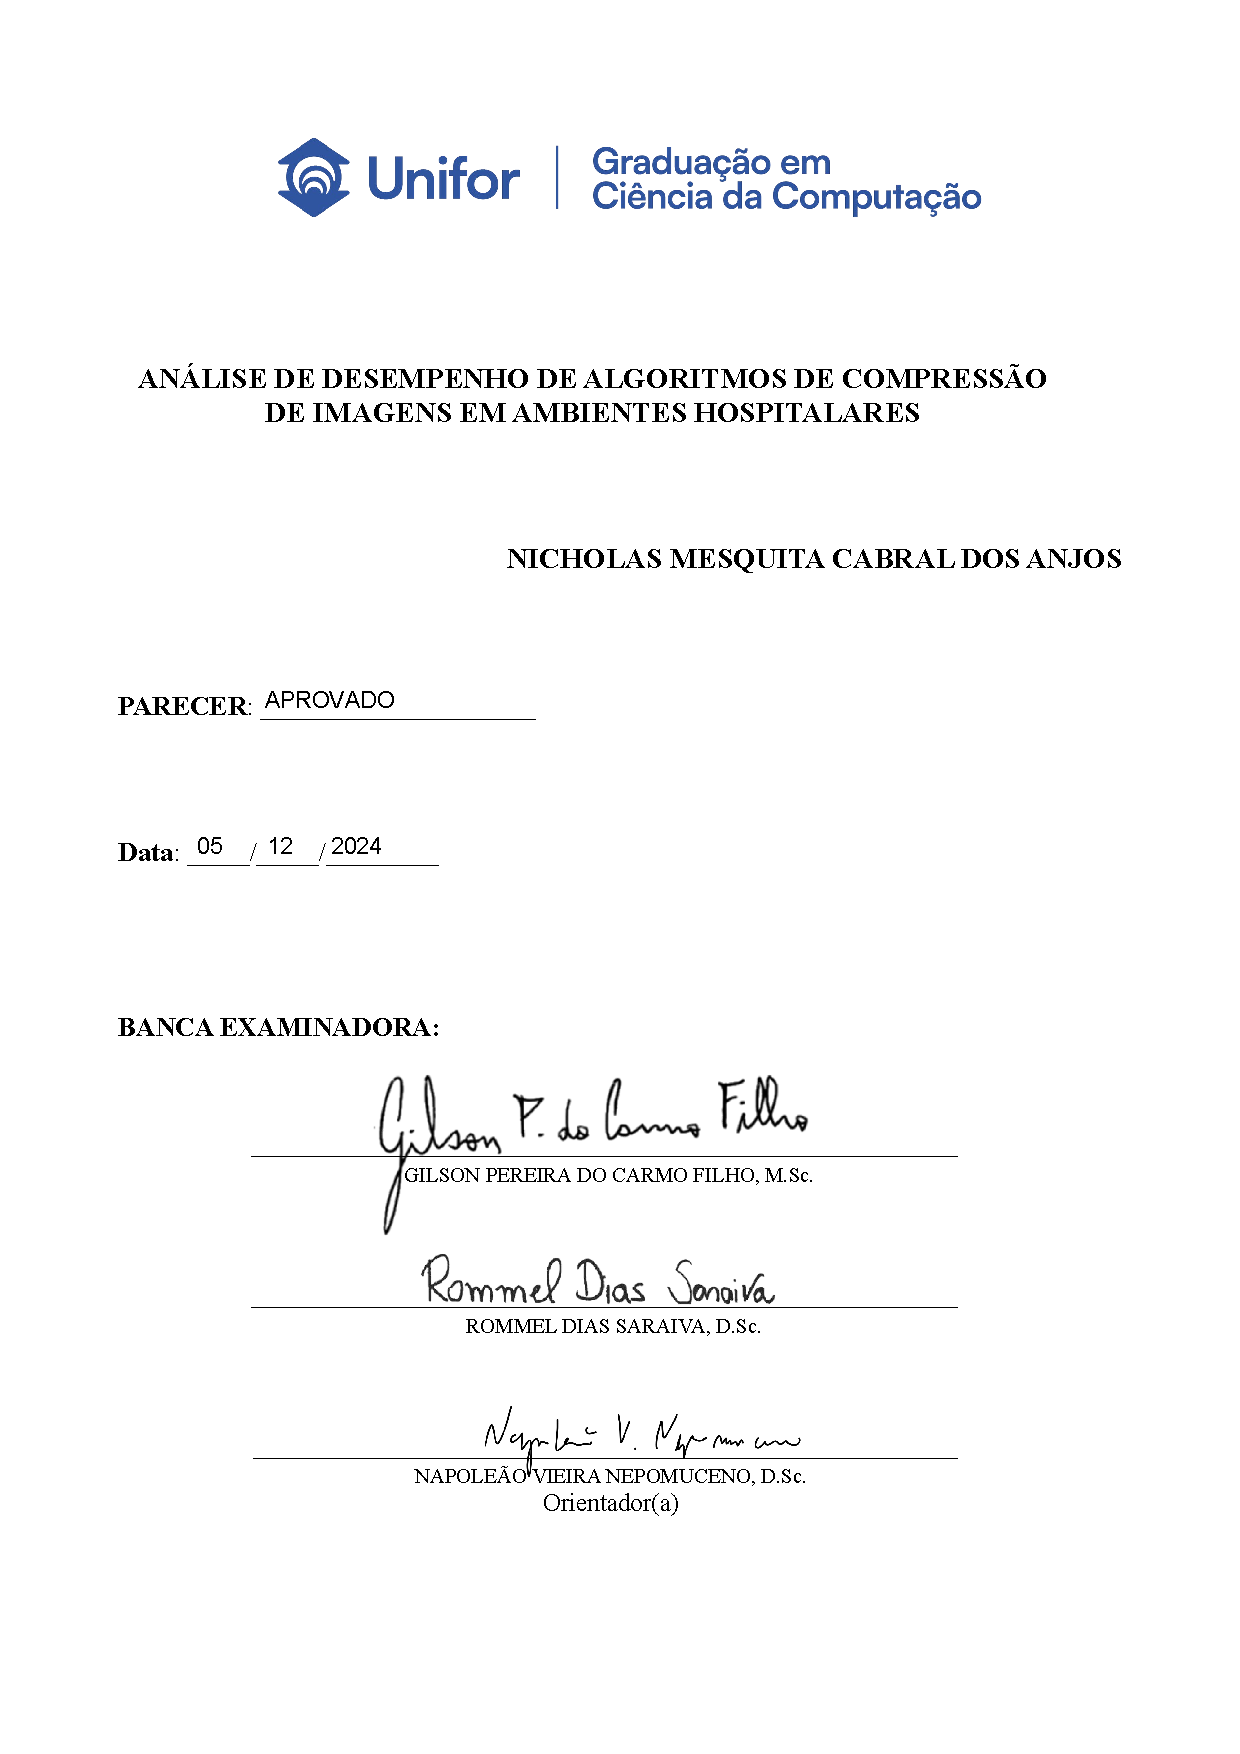
\includepdf{elementos-pre-textuais/folha-aprovacao.pdf} 		%%
	%%					removendo o simbolo de %													%%
	%%			6 - Adicione o simbolo % na linha 	\imprimirfolhadeaprovacao						%%
	%%			7 - Recompile o projeto																%%
	%%																								%%	%%%%%%%%%%%%%%%%%%%%%%%%%%%%%%%%%%%%%%%%%%%%%%%%%%%%%%%%%%%%%%%%%%%%%%%%%%%%%%%%%%%%%%%%%%%%%%%%%%
	
	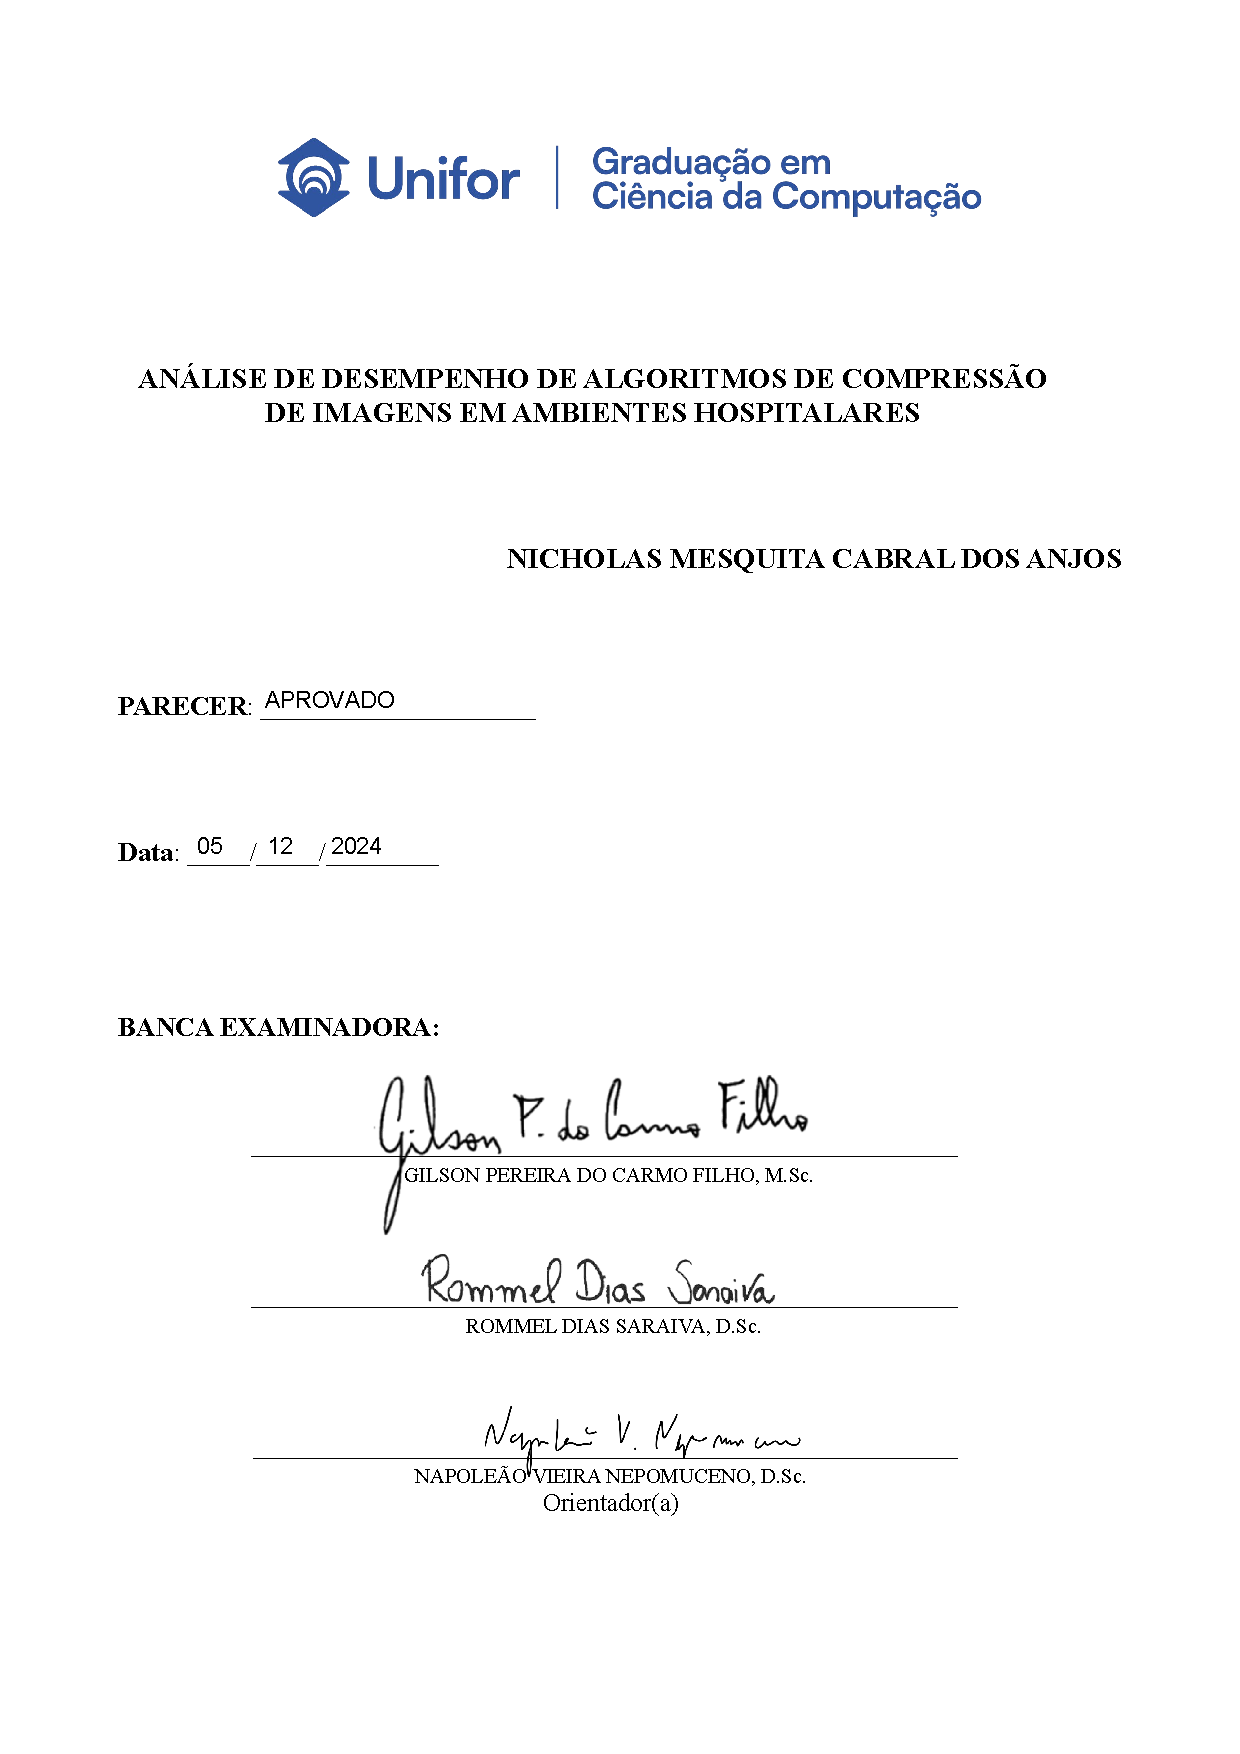
\includepdf{elementos-pre-textuais/folha-aprovacao.pdf}
	% \imprimirfolhadeaprovacao
	
	\imprimirdedicatoria{elementos-pre-textuais/dedicatoria}
	\imprimiragradecimentos{elementos-pre-textuais/agradecimentos}
	% \imprimirepigrafe{elementos-pre-textuais/epigrafe}
	\imprimirresumo{elementos-pre-textuais/resumo}
	\imprimirabstract{elementos-pre-textuais/abstract}
	\imprimirlistadeilustracoes
	% \imprimirlistadetabelas
	\imprimirlistadequadros
	\imprimirlistadealgoritmos
	% \imprimirlistadecodigosfonte
	\imprimirlistadeabreviaturasesiglas
	\imprimirlistadesimbolos{elementos-pre-textuais/lista-de-simbolos}
	\imprimirsumario

	% Elementos textuais
	\textual
	% \chapter{Introdução}
\label{cap:intro}

No âmbito da medicina, a obtenção e preservação de imagens de tomografia são desafios prementes. Por serem algo fundamental para os processos de análises radiológicas, é imprescindível que essas imagens tenham boa nitidez e praticidade de armazenamento. Com isso, a adoção do formato \acrfull{DICOM}
\cite{DICOM} como padrão internacional de imagens médicas aprimorou a forma como os hospitais lidam com as tomografias. O uso dessas imagens no cenário hospitalar, onde a complexidade dessas pode variar amplamente, resulta em arquivos que, em escala, podem sobrecarregar os sistemas de armazenamento dos hospitais. Este estudo compara métodos de compressão modernos para identificar formas eficientes de se armazenar essas imagens em diferentes cenários. 

\section{Definição do Problema}
\label{intro:prob}

A problemática essencial reside no gerenciamento eficaz de dados em ambientes hospitalares, onde várias tomografias são armazenadas, o que pode gerar um impacto substancial à infraestrutura digital dos hospitais. O volume crescente de dados gerados diariamente requer uma abordagem adaptativa para mitigar os desafios associados ao armazenamento e ao custo monetário elevado. Este estudo procura evidenciar \textbf{como diferentes métodos de compressão performam em diferentes cenários}, destacando suas vantagens e limitações, com o objetivo de compreender o impacto na integridade dos dados e auxiliar na escolha adequada para diferentes contextos de armazenamento.

\section{Motivação e Relevância}
\label{intro:motiv}

Este estudo é motivado pela necessidade de avaliar como diferentes métodos de compressão podem reduzir eficientemente o tamanho das imagens de tomografia, considerando o impacto na qualidade e identificando o equilíbrio entre compressão e preservação visual, tendo em vista sua importância na prática clínica. A tomografia desempenha um papel fundamental no diagnóstico e monitoramento de diversas condições médicas, e a compressão dessas imagens torna-se crucial para a manutenibilidade da infraestrutura digital dos hospitais. A relevância desta problemática está intrinsecamente ligada à crescente necessidade de tecnologias que melhorem o armazenamento e otimizem os recursos, visando eficiência e redução de custos. Ao comparar abordagens de compressão, temos como objetivo encontrar a forma que consiga conciliar uma alta taxa de compressão com uma baixa taxa de perda. Este estudo almeja ser uma contribuição para aprimorar a gestão de imagens de tomografia em ambientes hospitalares de grande escala.

\section{Objetivos}
\label{intro:objet}

O objetivo geral deste estudo é analisar o desempenho dos métodos de compressão \acrshort{PNG}, \acrshort{JPEG} e \acrshort{PCA} na redução do tamanho de imagens \acrshort{DICOM}, considerando diferentes tipos de órgãos (pulmão, mama e cérebro). A análise é realizada por meio da comparação das taxas de compressão e da perda de qualidade, buscando compreender como cada método concilia a redução do tamanho (em bytes) com a preservação da integridade das informações, em diferentes contextos de aplicação.

\subsection{Objetivos Específicos}
\begin{enumerate}
    \item Obter uma base de dados com imagens de tomografias.
    \item Implementar algoritmos modernos de compressão de imagens como \acrfull{PNG}, \acrfull{JPEG} e \acrfull{PCA}.
    \item Realizar um estudo comparativo entre os algoritmos citados acima.
    \item Investigar a relação entre as taxas de compressão e perda de qualidade de cada método.
    \item Identificar os cenários de armazenamento em que cada um dos métodos de compressão se mostra mais adequado, considerando as necessidades de eficiência no uso de espaço e preservação da qualidade das imagens médicas para diferentes tipos de órgãos.
    \item Explicar como cada órgão apresenta diferentes taxas de compressão, destacando as variações no desempenho dos métodos de compressão em função das características específicas de cada imagem.
\end{enumerate}

\section{Questões de Pesquisa}
\label{intro:questp}

% \begin{enumerate}
%     \item Quais são as taxas de compressão alcançadas pelos algoritmos \acrshort{PNG}, \acrshort{JPEG} e \acrshort{PCA} para imagens médicas de diferentes orgãos?
%     \item Quais métricas são adequadas para medir a perda de informações nas imagens após a compressão, e como essas métricas se aplicam aos diferentes algoritmos investigados?
%     \item De que forma a taxa de compressão impacta a qualidade visual das imagens de tomografia, considerando as características específicas de cada método de compressão?
% \end{enumerate}

\begin{enumerate}
    \item Quais são as taxas médias de compressão alcançadas pelos algoritmos \acrshort{PNG}, \acrshort{JPEG} e \acrshort{PCA} em imagens médicas de pulmão, mama e cérebro?
    \item Como as características das imagens de cada órgão (pulmão, mama e cérebro) influenciam as taxas de compressão dos algoritmos \acrshort{PNG}, \acrshort{JPEG} e \acrshort{PCA}?
    \item Como a variação da taxa de compressão impacta a qualidade visual das imagens de tomografia, considerando o \acrfull{PSNR} como métrica de avaliação?
    \item Qual algoritmo oferece o melhor equilíbrio entre compressão e qualidade visual para cada órgão, considerando os resultados de \acrshort{PSNR} e taxa de compressão?
\end{enumerate}

% \section{Contribuições do Trabalho}
% \label{intro:contr}
% \textbf{----- !!! FAZER DEPOIS !!! -----} 
% Texto indicando as contribuições do trabalho.
% \begin{enumerate}
%     \item \textbf{Avanço em pesquisas médicas:} \BlankLine
%     Ao oferecer uma análise detalhada e comparativa de métodos de compressão, o estudo contribui para o avanço da pesquisa médica, fornecendo insights sobre a eficácia desses métodos no contexto de armazenamento. O resultado dessa comparação pode orientar pesquisadores na escolha de métodos adequados para suas investigações.
    
%     \item \textbf{Aplicações de aprendizado de máquina:} \BlankLine
%     Muitas aplicações baseadas em IA dependem de grandes conjuntos de dados, incluindo imagens médicas. Imagens comprimidas facilitam o treinamento e a implantação mais rápidos de modelos. Pesquisadores e desenvolvedores que trabalham em algoritmos de IA para detecção, segmentação e classificação de doenças podem se beneficiar do armazenamento otimizado dessas imagens.

%     \item \textbf{Otimização de recursos:} \BlankLine
%     Hospitais e clínicas lidam diariamente com enormes quantidades de imagens médicas. A adoção de técnicas de compressão otimizadas pode resultar em economia significativa nos custos de armazenamento. Ao evidenciar o método mais eficiente dentre os mencionados acima, instituições de saúde podem se basear nesse resultado para a escolha do método de compressão mais adequado às suas necessidades específicas.
% \end{enumerate}

\section{Organização do Trabalho}
\label{intro:organ}
% \textbf{----- !!! FAZER DEPOIS !!! -----} O restante do trabalho está organizado nas seguintes seções. Na Capítulo~\ref{cap:fundamentacao-teorica}, apresenta-se a fundamentação teórica deste trabalho ...
O restante do trabalho está organizado nas seguintes seções:
\begin{itemize}
    \item No Capítulo~\ref{cap:fundamentacao-teorica}, são explorados os fundamentos teóricos essenciais da compressão de dados, uma área importante na ciência da computação e na transmissão eficiente de informações. São abordados os dois principais paradigmas de compressão: com perda e sem perda, discutindo os princípios subjacentes, as aplicações relevantes e as métricas comumente usadas para avaliar a eficácia de cada abordagem. O objetivo é fornecer uma base sólida para a análise detalhada dos algoritmos específicos de compressão e sua aplicação no contexto de otimização de imagens médicas.

    \item No Capítulo~\ref{cap:relac}, são discutidos estudos anteriores e pesquisas relevantes sobre a aplicação de técnicas de compressão de imagens em diferentes cenários, com ênfase no armazenamento de imagens de tomografia. A revisão da literatura existente identifica avanços, desafios e lacunas, contextualizando o estudo dentro do panorama atual da área e justificando a escolha dos algoritmos e metodologias utilizadas.

    \item No Capítulo~\ref{cap:metod}, são descritas detalhadamente as etapas e procedimentos adotados para a compressão de imagens de tomografia, incluindo a coleta de dados, a implementação dos algoritmos de compressão, a análise comparativa entre eles e a medição da perda de informações. São explicadas as ferramentas e técnicas utilizadas, justificadas as escolhas metodológicas e discutidas as considerações éticas e práticas associadas ao manejo dos dados de tomografia.

    \item No Capítulo~\ref{cap:resultados}, são apresentados os resultados obtidos, incluindo as taxas de compressão e de perda de qualidade alcançadas pelos algoritmos \acrshort{PNG}, \acrshort{JPEG} e \acrshort{PCA}. É analisada a perda de informações associada a cada método e seu impacto na qualidade das imagens, identificando os cenários mais adequados para a aplicação de cada técnica. Os dados obtidos são discutidos de maneira quantitativa e qualitativa, com gráficos e tabelas para ilustrar as descobertas.

    \item No Capítulo~\ref{cap:conclusao}, são apresentadas as conclusões finais, resumindo os principais achados e destacando as contribuições do estudo para a área de compressão de dados em imagens médicas. São discutidas as limitações encontradas durante a pesquisa e sugeridas direções para futuras investigações, com recomendações para o aprimoramento das técnicas de compressão e novas abordagens para a solução dos problemas identificados.
\end{itemize}


    % \item \textbf{Capítulo 1 - Introdução}:
    %  Neste capítulo introdutório, apresentamos a definição do problema relacionado ao gerenciamento eficaz de dados em ambientes hospitalares, focando na necessidade de armazenamento eficiente de imagens de tomografia. Discutimos a motivação e relevância do estudo, destacando a importância da compressão de dados para melhorar o armazenamento e transmissão dessas imagens. Os objetivos gerais e específicos são delineados, assim como as questões de pesquisa que nortearam a investigação. Detalhamos a metodologia adotada, as contribuições esperadas para a área e a estrutura do documento, proporcionando uma visão clara do conteúdo e da abordagem do trabalho.



	\chapter{Fundamentação Teórica}
\label{cap:fundamentacao-teorica}

Neste capítulo, serão explorados os fundamentos teóricos essenciais relacionados à compressão de dados, um campo vital na ciência da computação e na transmissão eficiente de informações. Abordamos os dois principais paradigmas de compressão, com perda e sem perda, discutindo os princípios subjacentes, as aplicações relevantes e as métricas comumente usadas para avaliar a eficácia de cada abordagem. Esses conceitos fundamentais são essenciais para compreender em detalhes os algoritmos específicos de compressão e sua aplicação no contexto prático de otimização de imagens médicas.

\section{Compressão de Dados}
\label{sec:compressão-de-dados}
A compressão de dados é um campo essencial na área da tecnologia da informação que visa reduzir o espaço de armazenamento e a largura de banda necessária para transmissão de informações sem comprometer a integridade dos dados. A Figura~\ref{fig:compression-example} ilustra a comparação de tamanho entre uma imagem original e uma imagem comprimida. O primeiro contato  significativo com a compressão de dados foi com a codificação de Huffman em 1952 \cite{huffmanArticle}, marco fundamental que estabeleceu as bases teóricas para a eficiente representação de informações.

\begin{figure}[!htbp]
	\centering
	\UNIFORfig{
	    \Caption{\label{fig:compression-example} Exemplo de compressão de imagem.}
	}{
	    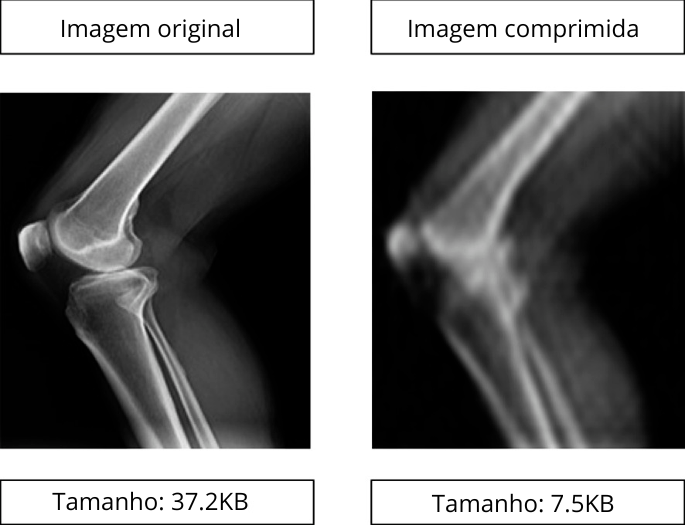
\includegraphics[width=0.55\textwidth]{images/compression-example.png}
	}{
	    \Fonte{Adaptada de \cite{imageCompressionExample}}
	}	
\end{figure}

\subsection{Taxa de compressão}
A taxa de compressão, ou do inglês \acrfull{CR}, é uma métrica crucial que quantifica a eficiência do processo de compressão. Ela é definida como a razão entre o tamanho do arquivo comprimido (\(S_{\text{comprimido}})\) e o tamanho do arquivo original (\(S_{\text{original}})\):
\begin{center}
    \(\displaystyle CR = 1 - \frac{S_{\text{comprimido}}}{S_{\text{original}}}\)
\end{center} 

\noindent A Figura~\ref{fig:compression-ratio-example} ilustra um exemplo dessa taxa de compressão, no qual é possível perceber que, à medida que a taxa de compressão aumenta, o tamanho do arquivo diminui, resultando em perdas progressivas de qualidade da imagem. Grosso modo isso se da pois quanto mais detalhes uma imagem tem, mais bits são necessários para representar aquela imagem. Isso é evidente na comparação visual entre a imagem original e suas versões comprimidas.

\begin{figure}[!htbp]
	\centering
	\UNIFORfig{
	    \Caption{\label{fig:compression-ratio-example} Comparação entre diferentes taxas de compressão}
	}{
	    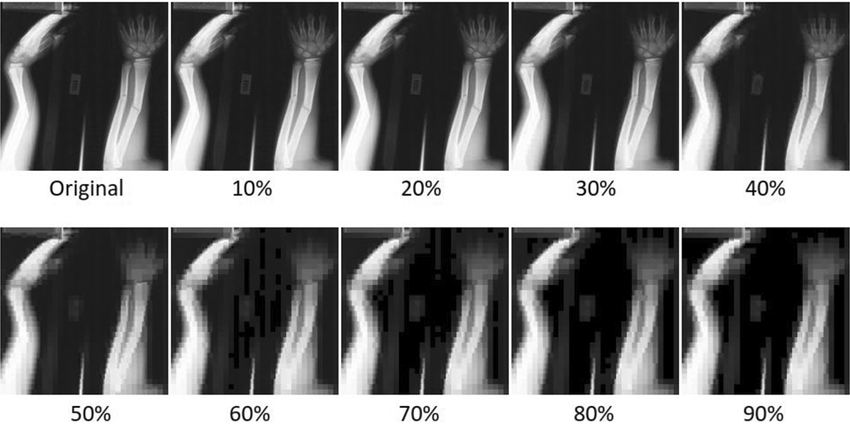
\includegraphics[width=\textwidth]{images/compression-ratio-example.png}
	}{
	    \Fonte{\cite{imageCompressionRate}}
	}	
\end{figure}
Quando falamos de compressão de dados, temos duas abordagens de algoritmos, os com perda e os sem perda, como ilustra a Figura~\ref{fig:lossless-vs-lossy}.

\begin{figure}[!htbp]
	\centering
	\UNIFORfig{
	    \Caption{\label{fig:lossless-vs-lossy} Comparação entre compressão com e sem perda}
	}{
	    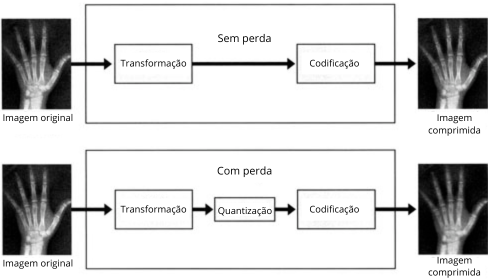
\includegraphics[width=\textwidth]{images/lossy-vs-lossless.png}
	}{
	    \Fonte{Adaptada de \cite{imageLossyVsLossless}}
	}	
\end{figure}

\subsection{Compressão sem perda}
A compressão sem perda preserva totalmente a informação original, explorando apenas a redundância dos dados e garantindo que a descompressão resulte no arquivo idêntico ao original. O algoritmo de Huffman \cite{huffmanArticle} é um exemplo clássico que utiliza códigos de comprimento variável para representar dados com diferentes frequências de ocorrência. Em outras palavras, em vez de atribuir um número fixo de bits para cada símbolo (como é o caso dos códigos de comprimento fixo), os códigos de comprimento variável permitem que símbolos mais comuns sejam representados por sequências de bits mais curtas, enquanto símbolos menos frequentes são representados por sequências de bits mais longas \cite{compressionTechniquesElakkiya}. Isso resulta em uma representação mais eficiente dos dados, uma vez que os símbolos mais comuns são codificados com menos bits, enquanto ainda mantém a capacidade de recuperar integralmente as informações originais durante o processo de descompressão. Essa abordagem de compressão é preferível em cenários em que nenhuma perda de integridade do documento é aceitável, como aqueles que envolvem documentos legais ou arquivos executáveis.

\subsection{Compressão com perda}
A compressão com perda, por outro lado, sacrifica parte da informação para obter uma maior taxa de compressão. Essa técnica é frequentemente empregada quando uma perda mínima de qualidade é aceitável para reduzir significativamente o tamanho do arquivo. Um exemplo comum é a compressão \acrshort{JPEG}. Ao contrário da compressão sem perda, que preserva integralmente as informações, a compressão com perda é mais flexível em relação à perda de informações. Ela é amplamente utilizada em cenários onde a qualidade ligeiramente inferior é aceitável em troca de uma redução significativa no tamanho do arquivo. Isso inclui aplicações como \textit{streaming} de vídeo, videoconferência e armazenamento de fotos em \textit{smartphones}. Para medir a perda resultante dessa compressão, uma métrica comumente empregada é o \acrfull{MSE}, que quantifica a diferença entre os valores originais e os valores comprimidos \cite{compressionTechniquesElakkiya}. A fórmula do \acrshort{MSE} é dada por:
\begin{center}
    \(\displaystyle MSE = \frac{\sum_{i=1}^{n} (X_i - Y_i)^2}{n}\)
\end{center}
\BlankLine
\noindent onde $n$ representa o número total de símbolos ou dados a serem comprimidos. A expressão \( \sum_{i=1}^{n} \) denota a soma dos termos, em que cada termo, $(X_i - Y_i)^2$, corresponde à diferença ao quadrado entre o valor original $X_i$ e o valor reconstruído $Y_i$ após a compressão. Essa operação garante que todas as diferenças sejam positivas e destaca as discrepâncias maiores entre os valores originais e os valores reconstruídos.

Além do \acrshort{MSE}, outra métrica comum para avaliar a perda de informações durante a compressão é a \acrfull{PSNR}. A \acrshort{PSNR} é frequentemente utilizada para medir a qualidade percebida da imagem após a compressão, fornecendo uma avaliação mais intuitiva para os usuários. A fórmula da \acrshort{PSNR} é dada por \cite{compressionTechniquesElakkiya}:
\begin{center}
    \(\displaystyle PSNR = 10 \cdot \log_{10}\left(\frac{\text{Valor Máximo}^2}{\text{MSE}}\right)\)
\end{center}
\BlankLine
Aqui, o Valor Máximo representa o maior valor possível de um pixel, geralmente representado pelo valor máximo que pode ser representado na imagem. Uma PSNR mais alta indica uma menor perda de informações e uma qualidade visual mais preservada. Essas métricas, como \acrshort{MSE} e \acrshort{PSNR}, fornecem maneiras objetivas de quantificar a perda de qualidade durante a compressão de dados, sendo ferramentas essenciais na avaliação do desempenho de algoritmos de compressão com perda.

\subsection{Entropia}
No contexto de compressão de imagem, a entropia é uma medida estatística que se refere à incerteza ou aleatoriedade das informações contidas em uma imagem. Quanto maior a entropia, mais imprevisíveis são os dados e mais difícil é comprimi-los. A entropia é frequentemente utilizada para  avaliar a eficiência da compressão sem perda, já que uma alta entropia implica em menor redundância nos dados, o que pode limitar a capacidade de compressão. A entropia de um conjunto de dados é calculada usando a teoria da informação de Shannon \cite{dataCopressionSayood}, sendo definida como a média ponderada das probabilidades dos símbolos no conjunto de dados. Matematicamente, a entropia de Shannon em bits $H(X)$ de uma variável aleatória discreta $X$ com distribuição de probabilidade $P(X)$ é definida por:
\BlankLine
\begin{center}
    \(\displaystyle H(X) = - \sum_{i=1}^{n} p(x_i) \log_2 p(x_i)\)
\end{center}

\noindent Onde $p(x_i)$ é a probabilidade do símbolo $(x_i)$ ocorrer no conjunto de dados.

Em imagens, a entropia é uma medida de quantidade de informação contida na imagem. Imagens com alta entropia tem uma maior variedade de cores e textura, o que torna mais difícil encontrar padrões repetidos e redundâncias que podem ser explorados para compressão, enquanto que imagens com baixa entropia têm menos variação e podem ser mais facilmente comprimidas. 

\subsection{\acrfull{DCT}}
A \acrfull{DCT} é uma técnica essencial na compressão de imagens, particularmente em algoritmos como o \acrshort{JPEG}. Ela desempenha um papel crucial ao converter os dados espaciais, ou seja, as informações sobre  a intensidade luminosa de cada pixel e sua localização na imagem em dados de frequência. Essa transformação é realizada por meio de uma série de operações matemáticas que convertem a informação de pixel em componentes de frequência \cite{digitalImageProcessingGonzalez}.

A \acrshort{DCT} divide a imagem em pequenos blocos e é aplicada a cada bloco separadamente. Durante esse processo, os padrões de variação são analisados na intensidade dos pixels dentro de cada bloco e são expressos em termos de frequência. Isso significa que a transformada identifica quais frequências estão presentes na imagem e em que intensidade, onde coeficientes de frequência de alta amplitude representam componentes de imagem que contribuem significativamente para a aparência visual, enquanto coeficientes de baixa amplitude representam detalhes menos perceptíveis. A definição da \acrshort{DCT} é dada por \cite{digitalImageProcessingGonzalez}:
\BlankLine
\begin{center}
    \(\displaystyle F(u,v) = \frac{1}{\sqrt{2N}}C(u)C(v)\sum_{x=0}^{N-1}\sum_{y=0}^{N-1}f(x,y)\cos\left[\frac{(2x + 1)u\pi}{2N}\right]\cos\left[\frac{(2y + 1)v\pi}{2N}\right]\)
\end{center}
\noindent onde $F(u,v)$ é o coeficiente da transformada na posição $(u,v)$, $f(x,y)$ é o valor do pixel na posição $(x,y)$, $N$ é o tamanho da imagem $C(u)$ e $C(v)$ são coeficientes de normalização. A expressão matemática da \acrshort{DCT} descreve como a transformação é realizada mapeando os valores de intensidade dos pixels para coeficientes de frequência, concentrando a energia da imagem nos coeficientes  de frequência mais significativos e descartando ou reduzindo os coeficientes de frequência de baixa amplitude

\subsection{Quantização}
A quantização é uma etapa essencial da compressão de imagem, que depende diretamente da \acrshort{DCT}. Após a aplicação da \acrshort{DCT}, os coeficientes de frequência resultantes são quantizados para reduzir a quantidade de dados necessários para representar a imagem. Esta etapa é critica, pois determina o nível de perda de qualidade que ocorrerá na imagem comprimida. A quantização é realizada dividindo-se os coeficientes de frequência pelos valores correspondentes na matriz de quantização e arredondando os resultados para o valor mais próximo. Isso resulta na perda de informações menos importantes da imagem, o que leva a uma redução significativa no tamanho da imagem \cite{quantizationGersho}.

A matriz de quantização controla o nível de compressão e, consequentemente, a taxa de perda de qualidade. Ao ajustar os valores na matriz de quantização, é possível parametrizar a compressão para comprimir mais ou menos. Reduzir os  valores na matriz de quantização resulta em uma compressão mais agressiva, o que leva a uma maior perda de qualidade na imagem comprimida. Por outro lado, aumentar os valores na matriz de quantização produz uma compressão menos agressiva, preservando mais detalhes na imagem. A quantização é definida por: 
\BlankLine
\begin{center}
    \(\displaystyle F_q(u,v) = \text{round}\left(\frac{F(u,v)}{Q(u,v)}\right) \)
\end{center}

\noindent Onde \textit{\(F_q\)(u,v)} é o coeficiente de frequência quantizado, $F(u,v)$ é o coeficiente de frequência original obtido pela \acrshort{DCT}, e $Q(u,v)$ é o valor correspondente na matriz de quantização. Essa equação exemplifica como a quantização é realizada, ajustando os coeficientes de frequência para reduzir a quantidade necessária de dados para  representar a imagem \cite{quantizationGersho}. A Figura~\ref{fig:quantization-example} compara três diferentes níveis de quantização, demonstrando como o aumento da quantização, ou seja, a diminuição de dados necessários para representar a imagem, afeta a nitidez, os detalhes e a fidelidade visual da imagem comprimida. 

\begin{figure}[H]
	\centering
	\UNIFORfig{
	    \Caption{\label{fig:quantization-example} Comparação entre diferentes níveis de quantização}
	}{
	    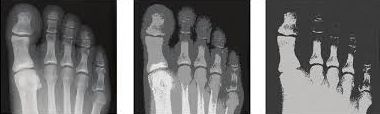
\includegraphics[width=\textwidth]{images/quantization-example.png}
	}{
	    \Fonte{Adaptada de \cite{imageQuantization}}
	}	
\end{figure}

\subsection{\acrfull{RGB} vs Escala de cinza (Grayscale)}
Imagens em \acrfull{RGB} são compostas por três canais de cores: vermelho, verde e azul. Cada pixel na imagem é representado por uma combinação desses três canais, onde a intensidade de cada canal determina a cor específica desse pixel. Geralmente, cada canal é representado por 8 bits, o que significa que cada canal pode ter 256 valores diferentes de intensidade, variando de 0 a 255. Portanto, uma imagem RGB típica possui 24 bits, ou 3 bytes, por pixel (8 bits para cada canal), resultando em uma gama de cores muito ampla e uma representação rica da imagem \cite{digitalImageProcessingGonzalez}.

Por outro lado, as imagens em escala de cinza são compostas por apenas um canal de intensidade luminosa, onde a cor de cada pixel é representada por um único valor de intensidade. Cada pixel em uma imagem em escala de cinza é representado por um valor de 8 bits, variando de 0 a 255, onde 0 representa preto e 255 representa branco \cite{digitalImageProcessingGonzalez}. Essa representação simplificada é adequada para imagens médicas, como as tomografias, onde a ênfase está na intensidade do sinal em vez das cores.

As imagens em escala de cinza requerem menos espaço de armazenamento e processamento computacional em comparação com as imagens RGB, o que é vantajoso ao lidar com grandes conjuntos de dados de tomografia. Portanto, ao analisar imagens de tomografia, é comum utilizar imagens em escala de cinza para representar com precisão as informações médicas relevantes.

\begin{figure}[H]
	\centering
	\UNIFORfig{
	    \Caption{\label{fig:rgb-grayscale-example} Visualização de uma imagem em escala de cinza e \acrshort{RGB}}
	}{
	    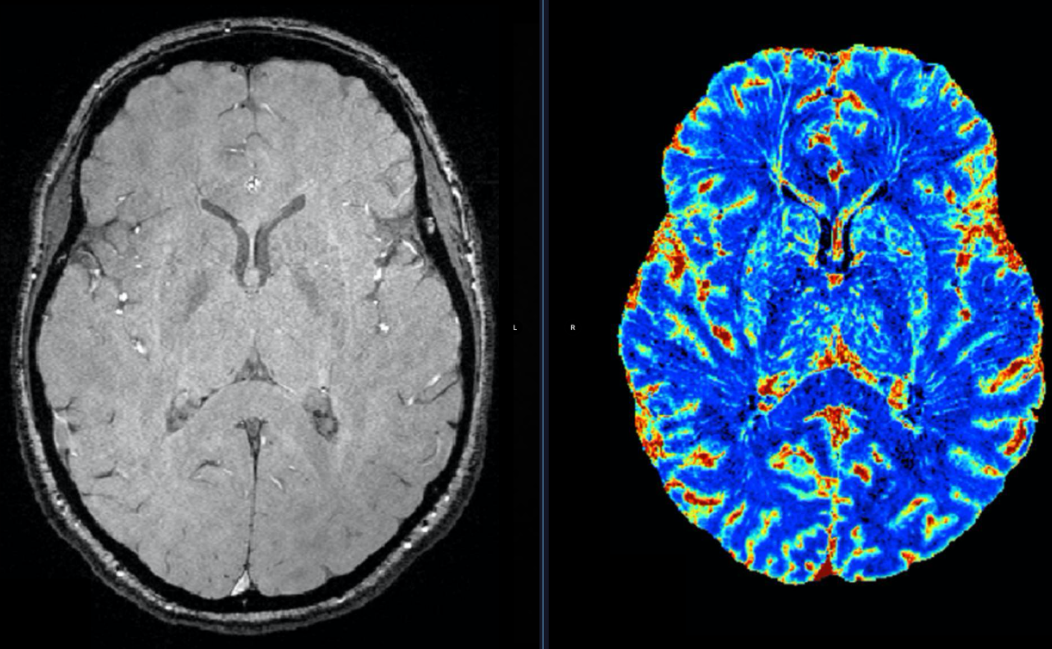
\includegraphics[width=\textwidth]{images/rgb-grayscale-example.png}
	}{
	    \Fonte{Extraída de \cite{imageRgbGrayscale}}
	}	
\end{figure}


\section{\acrfull{DICOM}}
O \acrshort{DICOM} é um padrão internacional fundamental para o armazenamento, transmissão e troca de informação de imagens médicas digitais \cite{DICOM}. Além de fornecer um formato padronizado, o \acrshort{DICOM} também estabelece diretrizes para metadados associados, como informações de paciente, estudo, série e imagem, como ilustrado na Figura~\ref{fig:dicom-metadata}. Uma característica distintiva das imagens \acrshort{DICOM} é a inclusão desses metadados detalhados, que permitem uma melhor compreensão e interpretação das imagens no contexto clínico.

Uma imagem é considerada \acrshort{DICOM} quando segue as especificações do padrão \acrshort{DICOM}, incluindo a estrutura de metadados e os requisitos de formato de arquivo. Essas imagens podem ser adquiridas por uma variedade de dispositivos médicos, como tomógrafos, ressonâncias magnéticas e sistemas de ultrassom, e são comumente usadas em diagnósticos por imagem, planejamento de tratamento e monitoramento de pacientes.

Quanto à compressão, as imagens \acrshort{DICOM} podem ser armazenadas em formato comprimido ou não comprimido, e essa informação é incluída nos metadados da imagem através do atributo \textit{TransferSyntaxUID}, onde este indica o esquema de codificação ou compressão de dados aplicado a uma imagem ou conjunto de dados \acrshort{DICOM}, e a ausência desse campo indica que a imagem não está comprimida \cite{DICOM}.

Embora seja amplamente adotado, ele tende a gerar arquivos volumosos devido aos metadados detalhados. Isso representa um desafio para o armazenamento eficiente, especialmente em ambientes hospitalares. A compressão de imagens \acrshort{DICOM} é uma solução, mas pode impactar na qualidade diagnóstica, especialmente com compressão com perda. É essencial encontrar um equilíbrio entre a redução do tamanho dos arquivos e a preservação da qualidade das imagens para garantir diagnósticos precisos e tratamentos eficazes na prática clínica. A Figura~\ref{fig:dicom-example} ilustra a visualização de uma imagem \acrshort{DICOM}.

\begin{figure}[H]
	\centering
	\UNIFORfig{
	    \Caption{\label{fig:dicom-metadata} Metadados de uma imagem \acrshort{DICOM}}
	}{
	    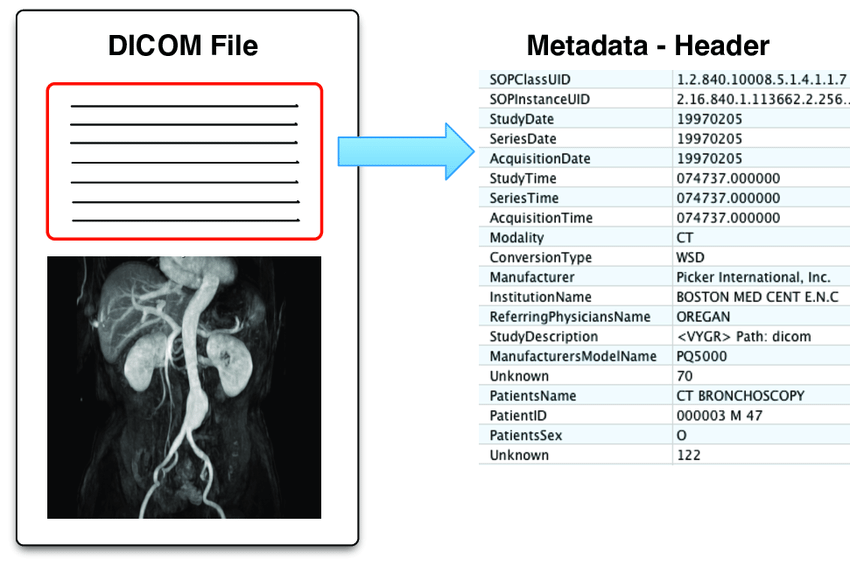
\includegraphics[width=\textwidth]{images/dicom-metadata.png}
	}{
	    \Fonte{Extraída de \cite{imageDicomMetadata}}
	}	
\end{figure}

\begin{figure}[H]
	\centering
	\UNIFORfig{
	    \Caption{\label{fig:dicom-example} Visualização de uma imagem \acrshort{DICOM}}
	}{
	    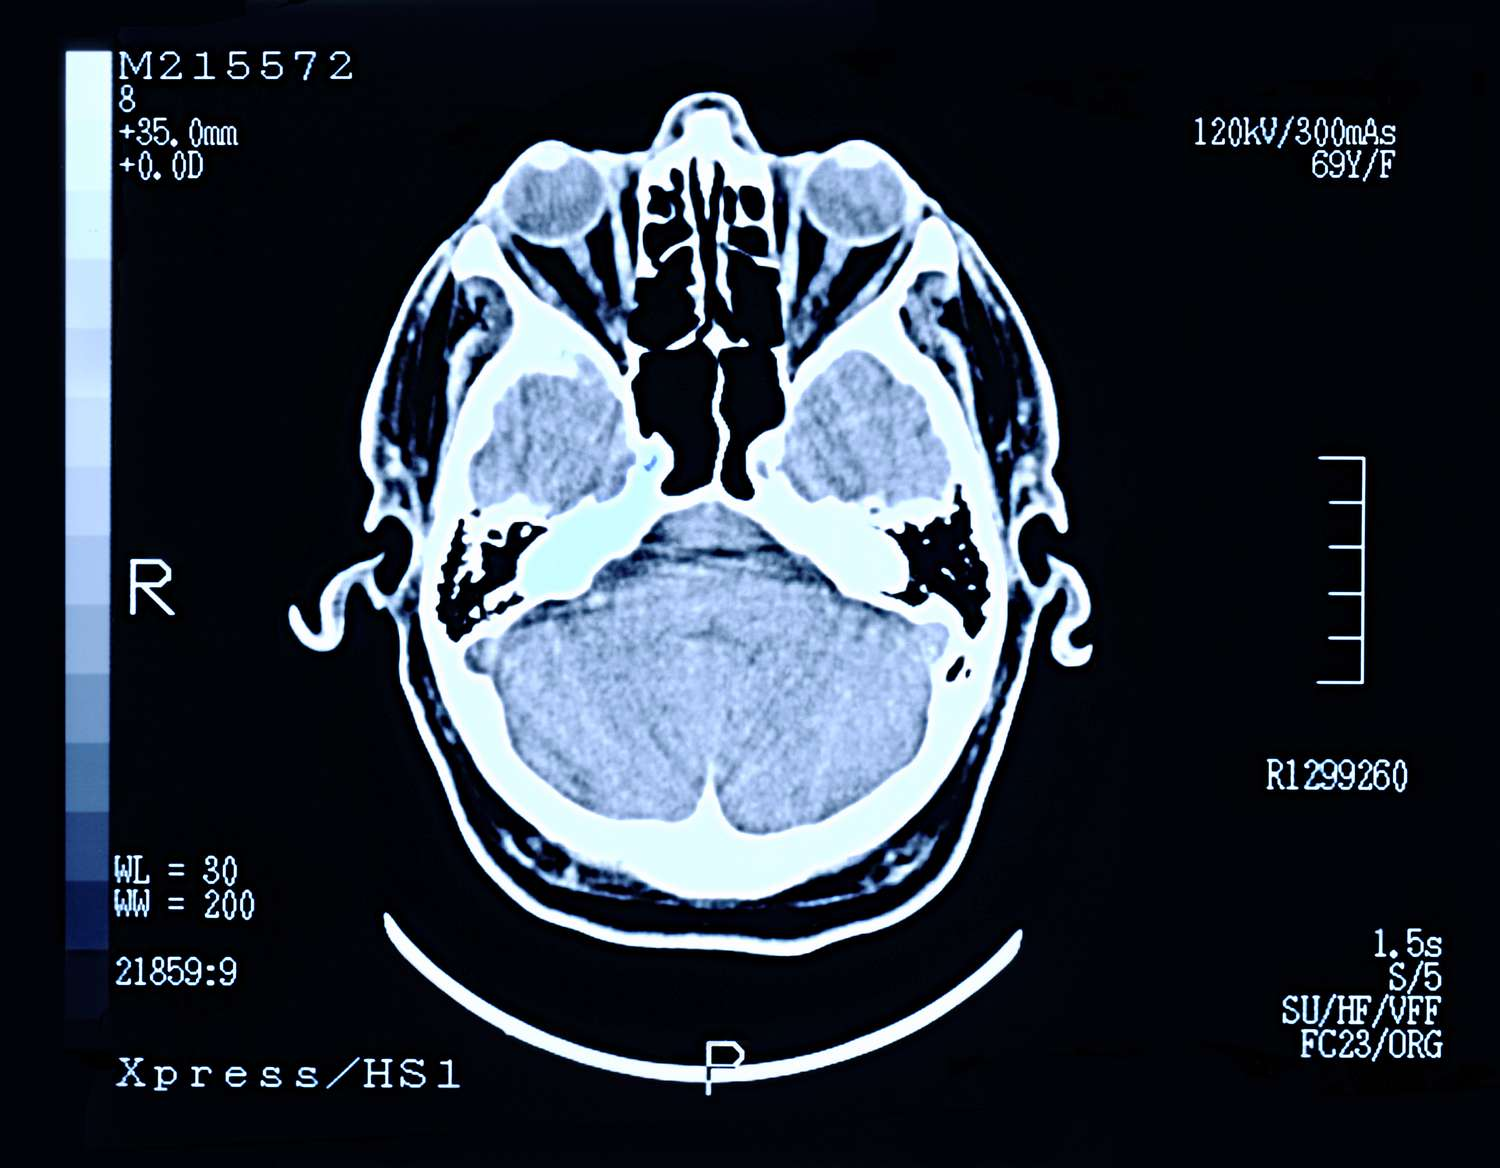
\includegraphics[width=\textwidth]{images/dicom-example.jpg}
	}{
	    \Fonte{Extraída de \cite{imageDicom}}
	}	
\end{figure}

\section{Algoritmo de Huffman}
O algoritmo de Huffman \cite{huffmanArticle} é um método de compressão sem perda que utiliza codificação de comprimento variável para representar símbolos de entrada com base em suas frequências de ocorrência. Desenvolvido em 1952 por David A. Huffman, esse algoritmo tem sido amplamente utilizado em uma variedade de aplicações de compressão de dados.

\begin{figure}[!htbp]
    \centering
    \UNIFORfig{
        \Caption{\label{fig:huffman-coding} Árvore de Huffman para uma sequência de caracteres aleatórios}
    }{
        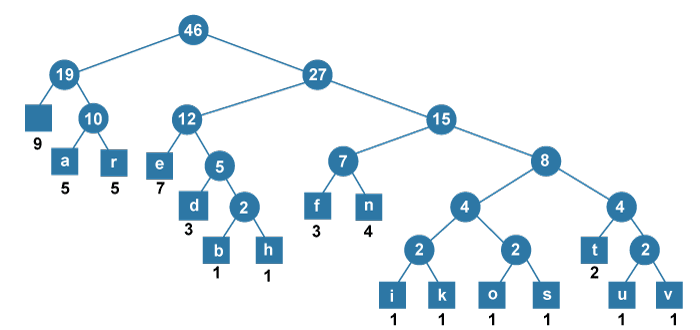
\includegraphics[width=\textwidth]{images/huffman-coding.png}
    }{
        \Fonte{\cite{imageHuffmanTree}}
    }   
\end{figure}

Para fins de ilustração, na Figura~\ref{fig:huffman-coding}, podemos ver que o símbolo ``a'' possui 5 ocorrências, enquanto o símbolo ``v'' possui apenas uma, então o caminho (quantidade de bits) para se representar o ``a'' é menor do que para se representar o ``v''.

O processo de compressão consiste nas seguintes etapas:
\begin{enumerate}
    \item Leitura dos dados de entrada:
    \BlankLine
    Todo o conteúdo do arquivo é lido do disco e armazenado na memória para manipulação posterior. Este passo é estratégico para o desempenho do algoritmo, pois permite que os dados sejam processados de forma eficiente. Uma abordagem alternativa seria processar os dados diretamente no arquivo, mas isso poderia resultar em perda de desempenho, especialmente para arquivos muito grandes.
    
    \item Construção da Fila de Prioridade:
    \BlankLine
    Nesta etapa do algoritmo de Huffman, os dados são utilizados para criar uma fila de prioridade com base na frequência de ocorrência dos símbolos presentes no texto original. Essa fila de prioridade é uma estrutura de dados que organiza os elementos de acordo com sua relevância, garantindo que os símbolos mais frequentes, que tendem a ter códigos mais curtos, sejam processados primeiro durante a construção da árvore de Huffman. Cada vez que um novo símbolo é encontrado no texto original, um nó é criado na fila de prioridade. Se o símbolo já está presente na fila, sua frequência é incrementada e o nó correspondente é reordenado na lista.

    \item Construção da Árvore Trie:
    \BlankLine
    A partir da fila de prioridade construída anteriormente, os dois nós de menor frequência (os dois primeiros) são removidos da fila e combinados para formar um novo nó que é reinserido na fila. Esse processo é repetido até que apenas um nó permaneça na fila, representando a raiz da árvore de Huffman. Esta árvore é ilustrada na Figura~\ref{fig:huffman-coding}.

    \item Construção da Tabela de Códigos:
    \BlankLine
    Uma vez construída a árvore de Huffman, uma tabela de códigos é criada para mapear cada símbolo ao seu código binário correspondente. Isso é feito percorrendo a árvore recursivamente, atribuindo códigos binários aos símbolos folha \cite{imeUspBinaryTrees}. Os símbolos mais frequentes recebem códigos mais curtos, enquanto os menos frequentes recebem códigos mais longos.

    \item Transformação do texto original em cadeia de bits:
    \BlankLine
    Utilizando a tabela de códigos, o texto original é transformado em uma cadeia de bits substituindo cada símbolo pelo seu código correspondente. Isso resulta em uma representação compacta do texto original, composta apenas por zeros e uns.

    \item Construção do fluxo de bytes comprimidos:
    \BlankLine
    A cadeia de bits gerada na etapa anterior é convertida em um fluxo de bytes comprimido, necessário porque os dados são armazenados em arquivos binários, e não diretamente como bits individuais.
\end{enumerate}

Uma das principais vantagens do algoritmo de Huffman \cite{huffmanArticle} é a sua capacidade de produzir uma representação compacta dos dados, especialmente para conjuntos de dados com distribuições de frequência desiguais. No entanto, a eficiência do algoritmo depende da capacidade de prever as frequências de ocorrência dos símbolos de entrada com precisão. Em alguns casos, a construção da árvore de Huffman pode ser computacionalmente intensiva, especialmente para conjuntos de dados grandes \cite{huffmanArticle}.

A complexidade de espaço do algoritmo de Huffman é dominada pelo tamanho da árvore de Huffman e pela tabela de códigos resultante, aproximadamente \( O(n) \) para uma árvore ótima, onde \( n \) é o número de símbolos distintos na entrada. Em termos de tempo, a construção da árvore de Huffman é \( O(n \log n) \) devido à combinação na fila de prioridade, enquanto a compressão dos dados é \( O(m) \), com \( m \) sendo o número total de bits no texto original. Essas características tornam o algoritmo de Huffman eficiente para compressão de dados em várias aplicações.

\begin{algorithm}[H]
\SetAlgoLined
\DontPrintSemicolon

\KwIn{Conjunto de caracteres e suas frequências}
\KwOut{Tabela de códigos de Huffman}

\BlankLine
Inicializar uma fila de prioridade $Q$ com os nós folha para cada caractere com sua frequência;
\While{$|Q| > 1$}{
$x \gets$ extrair o nó de menor frequência de $Q$;
\BlankLine
$y \gets$ extrair o próximo nó de menor frequência de $Q$;
\BlankLine
Criar um novo nó $z$ como nó interno com frequência $freq(z) = freq(x) + freq(y)$;
\BlankLine
$z$.esquerda $\gets x$;
\BlankLine
$z$.direita $\gets y$;
\BlankLine
Inserir $z$ de volta em $Q$;
}
Árvore de Huffman resultante é a única raiz restante em $Q$;
Derivar os códigos de Huffman percorrendo a árvore a partir da raiz;

\caption{Codificação de Huffman}
\end{algorithm}

\section{Algoritmos de compressão de imagens}
\subsection{\acrfull{PNG}}
\acrshort{PNG} é um formato de arquivo de imagem amplamente difundido que utiliza compressão sem perda de dados. A compressão \acrshort{PNG} é baseada no algoritmo DEFLATE \cite{dataCopressionSayood}, que é uma combinação de  dois outros algoritmos: \acrfull{LZ77} \cite{lempelZivArticle} e Huffman \cite{huffmanArticle}.
O processo de compressão de uma imagem para o formato \acrshort{PNG} consiste nas seguinte etapas:
\begin{enumerate}
    \item Pré-processamento:
    \BlankLine
    Antes da compressão, a imagem passa por um pré-processamento que pode incluir técnicas como o \textit{filtering prediction} \cite{compressionTechniquesElakkiya}. O \textit{filtering prediction} aplica filtros preditivos aos dados de imagem para estimar os valores dos pixels com base nos valores dos pixels vizinhos, ou seja, aqueles que estão na mesma linha ou coluna \cite{compressionTechniquesElakkiya}. Existem cinco tipos de filtros preditivos utilizados no formato PNG:
    \begin{itemize}
        \item Nenhum: Sem filtragem, os valores dos pixels são usados diretamente.
        \item Sub: O valor do pixel atual menos o valor do pixel anterior na linha.
        \item Up: O valor do pixel atual menos o valor do pixel acima na coluna.
        \item Average: A média dos pixels anterior na linha e acima na coluna subtraída do valor do pixel atual.
        \item Paeth: Um algoritmo que usa uma função preditiva para escolher o pixel mais próximo entre os pixels anterior, acima e a soma dos dois menos o pixel na diagonal superior esquerda.
    \end{itemize}
    O filtro de predição por subtração, por exemplo, pode ser representado pela seguinte fórmula:
    \begin{center}
        \(\displaystyle Pixel_{\text{predito}} = Pixel_{\text{atual}} - Pixel_{\text{vizinho}}\)
    \end{center}
    Ao aplicar esses filtros, a redundância nos dados de imagem é reduzida, o que aumenta a eficiência do algoritmo de compressão DEFLATE. Isso resulta em arquivos \acrshort{PNG} mais compactos e mais eficientes para armazenamento.

    \item Compressão com DEFLATE:
    \BlankLine
    O DEFLATE opera em duas principais etapas: a compactação com \acrshort{LZ77} e codificação de Huffman
    \begin{itemize}
        \item Compactação:
        O algoritmo \acrshort{LZ77} \cite{lempelZivArticle} procura por padrões repetidos de dados dentro de bloco. Ele substitui esses padrões por referências a cópias anteriores dos mesmos dados, seguido pela distância e pelo comprimento dessas cópias. Isso reduz a redundância nos dados e permite uma representação mais compacta.

        \item Codificação:
        Após a compactação, os dados da imagem são codificados usando o algoritmo de codificação de Huffman \cite{huffmanArticle}. Este atribui códigos mais curtos para padrões de pixels comuns, enquanto símbolos menos comuns, como detalhes finos ou ruído de imagem, recebem  códigos mais longos, resultando em uma representação mais eficiente, onde a informação visual é preservada de forma otimizada.
    \end{itemize}

    \item Estruturação em Chunks:
    \BlankLine
    A imagem \acrshort{PNG} é organizada em pedaços chamados "chunks". Cada chunk contém uma parte específica dos dados da imagem ou metadados. Os principais chunks incluem:

    \begin{itemize}
        \item IHDR: Contém informações básicas da imagem, como largura, altura, profundidade de cor e tipo de cor.
        \item IDAT: Contém os dados da imagem comprimidos.
        \item PLTE: Contém a paleta de cores, se aplicável.
        \item IEND: Indica o fim da imagem.
    \end{itemize}
    
\end{enumerate}
\BlankLine

\noindent As etapas de compressão do \acrshort{PNG}, como o pré-processamento, compressão com DEFLATE, e estruturação em chunks, são essenciais para reduzir o tamanho dos arquivos de imagem mantendo sua qualidade. \textit{filtering prediction} reduz a redundância, enquanto o DEFLATE proporciona uma compressão eficiente \cite{digitalImageProcessingGonzalez}. Essas etapas garantem arquivos compactos sem comprometer a qualidade da imagem.

\begin{figure}[!htbp]
	\centering
	\UNIFORfig{
	    \Caption{\label{fig:png-compression-example} Compressão de imagem com \acrshort{PNG}}
	}{
	    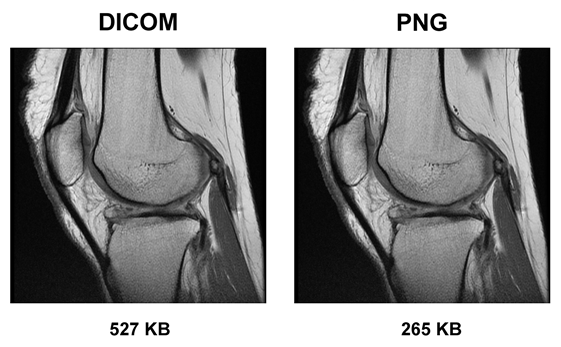
\includegraphics[width=\textwidth]{images/png-compression-example.png}
	}{
	    \Fonte{\cite{imagePNGCompression}}
	}	
\end{figure}

Considerando o desempenho da compressão \acrshort{PNG}, é crucial analisar tanto a complexidade de espaço quanto de tempo envolvida nesse processo. Em termos de complexidade de espaço, a quantidade de memória necessária para armazenar os dados intermediários durante a compressão e descompressão impacta diretamente no desempenho. Isso inclui a memória utilizada para manter as estruturas de dados para a fila de prioridade e a árvore de Huffman \cite{huffmanArticle}, bem como os \textit{buffers} para armazenar os dados comprimidos e descomprimidos. Além disso, a complexidade de tempo é influenciada pelo tamanho em bytes da imagem, uma vez que a aplicação dos algoritmos é realizada para a imagem inteira. Quanto maior o tamanho da imagem, mais tempo será necessário para processá-la. Todos esses fatores combinados podem impactar a complexidade de tempo e espaço da compressão \acrshort{PNG}. \cite{digitalImageProcessingGonzalez}


% JPG
\subsection{\acrfull{JPEG}}
\acrshort{JPEG} é um formato de compressão de imagens com perdas amplamente utilizado que emprega uma combinação de técnicas para reduzir o tamanho do arquivo, sem perder muita qualidade visual \cite{miano1999compressed}. Para imagens coloridas, o processo de compressão \acrshort{JPEG} envolve várias etapas fundamentais, incluindo a conversão de espaço de cores e \textit{downsampling}. No entanto, para imagens em escala de cinza, como elas possuem apenas um canal de cor (luminância) e não têm componentes de crominância, essas duas etapas não são necessárias \cite{digitalImageProcessingGonzalez}. Portanto, o processo de compressão \acrshort{JPEG} para imagens em escala  de cinza é simplificado em comparação com imagens coloridas. A Figura~\ref{fig:jpeg-flow} ilustra o processo de compressão e descompressão desse formato, as etapas principais incluem:

\begin{figure}[H]
	\centering
	\UNIFORfig{
	    \Caption{\label{fig:jpeg-flow} Fluxo de compressão e descompressão do \acrshort{JPEG}}
	}{
	    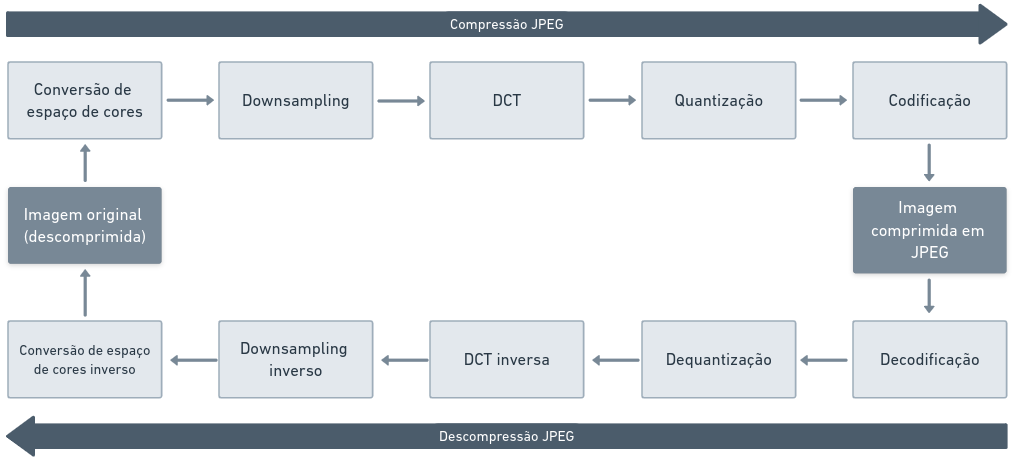
\includegraphics[width=\textwidth]{images/jpeg-flow.png}
	}{
	    \Fonte{Elaborado pelo autor}
	}	
\end{figure}

\begin{enumerate}
    \item Conversão de Espaço de Cores (\textit{Color Space Conversion}):
    Antes da compressão, a imagem é convertida de  seu espaço de cores original para outro espaço de cores mais adequado. Isso é especialmente importante para imagens em  escala de cinza, onde a conversão para um espaço de cores como o YCbCr pode melhorar a eficiência da compressão. No caso das imagens em escala de cinza, embora tenham apenas um canal de cor (luminância), a conversão para o espaço de cores YCbCr ainda pode ser benéfica. Isso ocorre porque a representação YCbCr separa a informação de luminância (Y) das informações de crominância (Cb e Cr), permitindo que a compressão se concentre principalmente na luminância, que é mais perceptível aos olhos humanos \cite{miano1999compressed}.

    \item \textit{Downsampling:}
    A etapa de \textit{downsampling} é usada para reduzir a resolução das componentes de crominância (Cb e Cr) mantendo a resolução da luminância (Y). Isso é feito porque as informações de cor nas imagens podem ser redundantes, especialmente nas componentes de crominância. No entanto, para imagens em escala de cinza, essa etapa é ignorada, pois não há informações de crominância para serem amostradas \cite{miano1999compressed}.

    \item \acrshort{DCT}:
    Após a conversão do espaço de cores e o \textit{downsampling}, cada bloco da imagem é submetido à transformada discreta do cosseno \acrshort{DCT}. Essa converte os dados espaciais da imagem em coeficientes de frequência, separando os componentes de alta e baixa frequência. Isso permite uma representação mais eficiente da imagem, concentrando a energia nos coeficientes de frequência mais significativos \cite{miano1999compressed}.

    \item Quantização:
    Os coeficientes de frequência resultantes da \acrshort{DCT} são quantizados para reduzir a quantidade de dados necessários para representar a imagem, Esta etapa introduz perda de qualidade, pois envolve a redução da precisão dos coeficientes de frequência menos significativos. A matriz de quantização é ajustada para controlar o nível de compressão e, consequentemente, a taxa de perda de qualidade \cite{miano1999compressed}.

    \item \textit{Run-Length Encoding} e \textit{Huffman Coding}:
    Após a quantização, os coeficientes de frequência quantizados são submetidos à codificação de \acrfull{RLE} e, em seguida, à codificação de Huffman \cite{huffmanArticle}. A codificação \acrshort{RLE} é utilizada para comprimir sequências de zeros consecutivos nos dados quantizados, enquanto a codificação de Huffman \cite{huffmanArticle} atribui códigos de comprimento variável aos símbolos com base em sua probabilidade de ocorrência. Essas técnicas de codificação contribuem para uma compressão eficiente dos dados, reduzindo ainda mais o tamanho da imagem \cite{miano1999compressed}.
\end{enumerate}

\noindent Essas etapas juntas compõem o processo de compressão \acrshort{JPEG}, que possibilita a redução do tamanho do arquivo de imagem com perdas controladas. Embora a qualidade da imagem seja comprometida devido à perda de informações durante a quantização, o algoritmo \acrshort{JPEG} oferece um equilíbrio adequado entre tamanho do arquivo e qualidade visual aceitável para uma ampla gama de aplicações \cite{digitalImageProcessingGonzalez}.

Considerando o desempenho da compressão \acrshort{JPEG}, é crucial analisar tanto a complexidade de espaço quanto de tempo envolvida nesse processo. Em termos de complexidade de espaço, a quantidade de memória necessária para armazenar os dados intermediários durante a compressão e descompressão impacta diretamente no desempenho. Isso inclui a memória utilizada para manter os blocos de pixels, as estruturas de dados para a fila de prioridade e as tabelas de Huffman, bem como os buffers para armazenar os dados comprimidos e descomprimidos. Além disso, a complexidade de tempo é influenciada pelo tamanho em bytes da imagem, uma vez que a compactação é realizada para cada bloco individualmente. Quanto maior o tamanho da imagem, mais blocos serão processados, aumentando assim a complexidade de tempo da compressão e descompressão \acrshort{JPEG}. Todos esses fatores combinados podem impactar a eficiência e o desempenho geral da compressão \acrshort{JPEG}.

\subsection{\acrfull{PCA}}
\acrfull{PCA} é uma técnica fundamental em análise de dados e  aprendizado de máquina amplamente utilizada para redução de dimensionalidade de dados \cite{multivariateAnalysis}. O \acrshort{PCA} é uma abordagem estatística que busca encontrar as direções de maior variabilidade nos dados, representadas pelos autovetores da matriz de covariância, e projetar os dados nesses componentes principais. Essa técnica tem aplicações em diversas áreas, incluindo reconhecimento de padrões, visão computacional e compressão de dados. As etapas principais dessa abordagem para compressão de imagens são:

\begin{enumerate}
    \item Preparação da imagem:
    A imagem é convertida para escala de cinza, reduzindo a quantidade de canais da imagem, mantendo apenas o canal de nível de cinza, sendo cada pixel representado por um valor entre 0 e 255, onde 0 é preto, e 255, branco \cite{multivariateAnalysis}.

    \item Organização dos dados:
    A matriz de pixels é convertida em um vetor unidimensional de tamanho $m \times n$, onde $m$ representa a quantidade  de linhas e $n$ a quantidade de colunas da matriz, ou seja, se a imagem tiver uma resolução de 512x512 o resultado seria um vetor unidimensional de tamanho 262.144 (512x512), onde cada elemento do vetor representa a intensidade do pixel em uma posição especifica da imagem \cite{multivariateAnalysis}.

    \item Centralização dos dados:
    Após a organização dos dados, é calculada a média de todos  os valores de intensidade dos pixels na imagem. O valor dessa média é subtraído de cada valor de pixel no vetor de dados. Isso centraliza  os dados em torno de zero, removendo a informação de brilho médio da imagem \cite{multivariateAnalysis}.

    \item Cálculo da matriz de covariância:
    A partir da centralização dos dados, é calculada a matriz de covariância. Covariância entre dois pixels indica como eles variam juntos, uma covariância positiva entre os pixels sugere que eles variam juntos na mesma direção, enquanto uma covariância negativa indica que eles variam em direções opostas. Isso ajuda a identificar as direções principais de variabilidade nos dados, que são representadas pelos autovetores da matriz de covariância. Essas direções principais são usadas para comprimir e reconstruir a imagem com perda mínima de informação \cite{multivariateAnalysis}.

    \item Decomposição da matriz  de covariância:
    Decompondo a matriz de covariância são obtidos os autovetores e autovalores. Onde os autovetores representam as direções principais de variabilidade nos dados, enquanto os autovalores indicam a quantidade de variância ao longo de cada uma dessas direções \cite{multivariateAnalysis}.

    \item Seleção dos componentes principais:
    Após a decomposição da matriz de covariância, os autovetores são ordenados de acordo com seus autovalores correspondentes, em ordem decrescente. Dessa forma, os autovetores com os maiores autovalores contêm a maior parte da variância dos dados e, portanto, são tratados como os componentes principais \cite{multivariateAnalysis}.

    \item Compressão:
    Nesta etapa, o algoritmo se torna parametrizável, permitindo que escolhamos a quantidade de componentes principais para representar a imagem. Em outras palavras, quanto menos componentes principais forem selecionados, maior será a taxa de compressão e menor será a qualidade da imagem resultante. Ao escolher a quantidade de componentes principais, é multiplicado o  vetor de dados centralizados pelos autovetores correspondentes aos $n$ maiores autovalores, onde $n$ é o número de componentes selecionados, e então é adicionado a média de volta ao vetor resultante. Isso constrói uma versão comprimida da imagem original em formato de vetor, mantendo apenas as informações mais relevantes em termos de  variabilidade de dados \cite{multivariateAnalysis}.

    \item Descompressão:
    Para reconstruir a imagem original, é multiplicada o vetor comprimido da imagem original pelos autovetores transpostos (ou seja, os autovetores originais), e então adicionada a média de volta para obter a imagem reconstruída \cite{multivariateAnalysis}.
    
\end{enumerate}
	\chapter{Trabalhos Relacionados}
\label{cap:relac}

Neste capítulo, apresentamos uma revisão dos trabalhos relacionados ao tema do nosso estudo. O objetivo é fornecer uma visão geral dos estudos anteriores que abordam questões semelhantes às que estamos investigando. Ao revisar esses trabalhos, buscamos identificar lacunas no conhecimento existente e destacar como nossa pesquisa contribui para preencher essas lacunas.

\section{Processos de Compressão de Dados Aplicados a Imagens Médicas} 
No estudo \citeonline{stolfi2000MedicalCompression}, o autor aborda a aplicação de técnicas de compressão de dados em imagens médicas, com foco específico na cineangiografia, uma técnica de imagem que registra o fluxo sanguíneo dentro dos vasos. Ele ressalta a importância da qualidade e fidelidade na reprodução das imagens médicas para diagnósticos precisos e procedimentos médicos. Reconhecendo a necessidade de altas taxas de compressão sem perdas, o autor destaca os desafios associados especialmente em imagens ruidosas.

Para abordar esses desafios, propõe-se a implementação de um sistema de compressão de imagem em movimento, com ênfase na cineangiografia. O autor desenvolve um processo de compensação de movimento baseado em semelhança de forma para otimizar a extração de vetores em movimento, visando melhorar tanto a taxa de compressão quanto a qualidade da imagem reconstruída em comparação com métodos tradicionais. Além disso, explora-se o uso de quantização não linear e pós-processamento das imagens reconstruídas para reduzir a visibilidade de erros introduzidos durante o processo de compressão. Destaca-se a importância da avaliação dos resultados por meio de um ambiente de visualização de imagens, permitindo comparações entre diferentes métodos de processamento.

Em resumo, o trabalho representa uma contribuição significativa para a área de compressão de dados em imagens médicas, uma vez que explora essas compressões para o contexto específico  da cineangiografia. 

\section{Compressão de Imagens Mamográficas Utilizando Segmentação e o Algoritmo \acrshort{PPM}}
A principal problemática abordada no artigo de \citeonline{marques2007mamografia} é a necessidade de  comprimir imagens mamográficas de forma eficiente, preservando informações essenciais para diagnósticos precisos. A digitalização de imagens mamográficas resulta em arquivos de grande tamanho, o que pode sobrecarregar os sistemas de armazenamento e dificultar a transmissão dessas imagens, impactando a eficiência dos processos médicos. Para solucionar essa questão, os autores propuseram um método que combina a segmentação por limiarização, a decomposição da imagem em planos de bits e a utilização do algoritmo de compressão \acrfull{PPM}. Essa abordagem permitiu alcançar taxas de compressão competitivas em relação a outros compressores avançados, ao mesmo tempo em que preservou a qualidade e a integridade das informações contidas na imagem original.

Em resumo, o estudo destaca a relevância da inovação tecnológica na área de compressão de imagens médicas, demonstrando  que a combinação dessas técnicas pode resultar em benefícios significativos para a área da saúde. Essa abordagem não apenas contribui para a otimização do armazenamento e transmissão de imagens mamográficas, mas também pode facilitar a análise e o compartilhamento desses dados, auxiliando profissionais de saúde em diagnósticos mais precisos e eficazes. 

% Meu estudo visa expandir as métricas eficiência de compressão de dados para imagens mamográficas, uma  vez que utiliza métodos de compressão modernos.


\section{Utilização da Análise de Componentes Principais na compressão de imagens digitais}
A problemática abordada por \citeonline{santos2012PCACompression} estava relacionada à necessidade de comprimir imagens médicas de forma eficiente, mantendo as informações essenciais para o diagnóstico clínico, ao mesmo tempo em que se reduz o espaço de armazenamento necessário. A compressão de imagens é crucial em ambientes médicos, onde grandes volumes de dados de imagem são gerados diariamente e o armazenamento eficiente é fundamental para a gestão e análise dessas informações. O autor explorou o \acrshort{PCA} como uma ferramenta estatística para redução da dimensionalidade dos dados de imagem. A aplicação do \acrshort{PCA} permitiu representar as imagens em uma estrutura computacional de dimensão reduzida, preservando as características principais da imagem original. Isso foi alcançado por meio da projeção dos dados em um subespaço gerado por um sistema de eixos ortogonais, obtido através do método \acrfull{SVD} \cite{santos2012PCACompression}.

Os resultados do estudo demonstraram que as imagens médicas comprimidas mantiveram suas principais características até aproximadamente $1/4$ do tamanho original, ou seja, uma taxa de compressão de aproximadamente 75\%, evidenciando a eficácia do \acrshort{PCA} como uma ferramenta de compressão de imagens. A quantidade de componentes principais utilizadas na compressão foi destacada como um fator crucial, pois influencia diretamente na recuperação da imagem original a partir da imagem compactada. A taxa de compressão obtida foi um aspecto chave, pois quanto maior a taxa de compressão (menos componentes principais utilizados), maior a degradação da qualidade da imagem recuperada.

Em resumo, o autor ressaltou a importância do \acrshort{PCA} como uma abordagem eficaz para a compressão de imagens médicas, proporcionando economia de espaço de armazenamento sem comprometer significativamente a qualidade das imagens. A consideração da quantidade de componentes principais na compressão foi destacada como um aspecto crucial para garantir a recuperação adequada das informações visuais essenciais nas imagens médicas comprimidas.

\section{Compressão de imagens com transmissão em tempo real}
No estudo de \citeonline{sousa2015compressaoTempoReal}, foi adotada a compressão com perdas, onde a qualidade visual da imagem pode ser comprometida em troca de uma maior eficiência na transmissão. Para minimizar o custo computacional exigido, foi escolhida a Transformada de Wavelet discreta de Haar \cite{sousa2015compressaoTempoReal}, que, apesar de não proporcionar a melhor qualidade de imagem, é mais eficiente em termos de processamento, sendo adequada para aplicações em tempo real. A utilização da Transformada de Wavelet de Haar aliada à quantização permitiu a redução da quantidade de dados redundantes na imagem, garantindo uma compressão eficaz. O estudo buscou atender a uma taxa de transmissão de 30 FPS (\textit{frames per second}), o que exigiu a realização da compressão e transmissão de cada imagem em menos de 33,333 milissegundos para assegurar a transmissão em tempo real.

% Portanto, reconhecemos a importância desse trabalho, que se concentrou na busca por métodos eficientes que permitissem a transmissão de imagens em tempo real. Considerando a necessidade de equilibrar a qualidade visual com a velocidade de transmissão, esse estudo oferece contribuições valiosas para aplicações que requerem resposta em tempo real, como em sistemas de monitoramento e diagnóstico médico.

\section{Projeto de Arquiteturas Integradas para a compressão de imagens \acrshort{JPEG}}
O trabalho de \citeonline{agostini2002JPEGArch} se concentra na compressão de imagens fotográficas digitais, especialmente utilizando o padrão \acrshort{JPEG}, amplamente reconhecido e utilizado para a compressão de imagens. A motivação principal é a redução dos dados de imagem para otimizar recursos de armazenamento e transmissão. No sistema de monitoramento de Porto Alegre, as imagens não comprimidas geram altos custos de armazenamento e transporte. Com a compressão \acrshort{JPEG}, o sistema poderia aumentar sua capacidade de armazenamento, reduzir custos operacionais e melhorar eficiência geral.

O autor desenvolve arquiteturas específicas para compressão de imagens em \textit{Grayscale} e \acrshort{RGB}, incluindo a conversão de imagens do espaço de cores \acrshort{RGB} para YCbCr. A solução proposta envolve o desenvolvimento de arquiteturas descritas em VHDL, direcionadas para síntese em FPGA's da Altera, permitindo um processamento mais rápido e eficiente. Para imagens em \textit{Grayscale}, a arquitetura pode processar uma imagem de $640x480$ pixels em 18.5ms, permitindo uma taxa de 54 imagens por segundo. Para imagens \acrshort{RGB}, a arquitetura pode processar uma imagem de $640x480$ pixels em 54.4ms, com uma taxa de 18.4 imagens por segundo e uma compressão estimada de 93\%.

Em resumo, o autor apresenta uma solução eficiente para a compressão de imagens \acrshort{JPEG}, com aplicações potenciais em sistemas de monitoramento de trânsito e outras áreas que demandam processamento rápido e eficiente de imagens. A pesquisa contribui significativamente para a área, pois sugere desenvolve uma forma mais eficiente para comprimir imagens tanto em \textit{Grayscale} quanto em \acrshort{RGB}.
	\chapter{Metodologia}
\label{cap:metod}

Neste capítulo, será detalhada a abordagem metodológica adotada para investigar  o desempenho dos algoritmos de compressão de imagem \acrshort{PNG}, \acrshort{JPEG} e \acrshort{PCA} no contexto de imagens de tomografia no formato \acrshort{DICOM}. A metodologia empregada busca não apenas comparar as taxas de compressão, mas também avaliar o impacto dessa compressão na qualidade das imagens. Para tanto, cada etapa do processo será minuciosamente descrita, desde a coleta e pré-processamento dos dados até a aplicação dos algoritmos de compressão e a análise dos resultados. O foco está em estabelecer uma compreensão clara e fundamentada das vantagens e limitações de cada método em cenários hospitalares.

\section{Base de dados}
\label{metod:dados}

Neste estudo, as imagens de tomografia foram obtidas do \acrfull{TCIA}, uma vasta coleção de imagens médicas voltada para pesquisas em oncologia. o \acrshort{TCIA} é um recurso público que disponibiliza imagens de alta qualidade, incluindo tomografias computadorizadas, ressonâncias magnéticas, e outros exames, coletados de pacientes com diversos tipos de câncer. O banco de dados é amplamente utilizado para pesquisas acadêmicas e desenvolvimento de algoritmos de análise de imagem.

O \acrshort{TCIA} é uma parte do \acrfull{NBIA}, uma iniciativa do \acrfull{NIH} dos Estados Unidos. o \acrshort{NBIA} foi criado para facilitar o compartilhamento de imagens biomédicas para pesquisa, oferecendo uma plataforma segura e padronizada para o armazenamento e disseminação de imagens médicas. A integração do \acrshort{TCIA} ao \acrshort{NBIA} garante que as imagens disponibilizadas estejam dentro dos padrões de qualidade e anonimidade exigidos para pesquisas científicas.

\subsection{Classificação das imagens}
Para este estudo, foram selecionadas 15.000 imagens de tomografia computadorizada provenientes de diferentes coleções de imagens do \acrfull{TCIA}, todas no formato \acrshort{DICOM}. A seleção das imagens foi realizada com base em um critério específico: de cada coleção, foram escolhidas 5.000 imagens com a mesma resolução. Essas imagens foram agrupadas em três tipos de câncer distintos, permitindo uma análise comparativa entre eles. Importante ressaltar que as imagens selecionadas não possuíam compressão prévia, o que garantiu a integridade dos dados para os testes de compressão realizados, mas esse aspecto será detalhado mais adiante. Os três tipos de câncer selecionados foram:

\begin{itemize}
    \item \textbf{Câncer de Mama}: As 5.000 imagens de câncer de mama foram adquiridas da coleção \acrfull{EA1141} \cite{breastCancerCollection}, disponível no The Cancer Imaging Archive em \url{https://www.cancerimagingarchive.net/collection/ea1141}. As imagens de mama geralmente contêm uma proporção significativa de tecido denso e menos espaços vazios, o que pode dificultar a compressão em relação a outros órgãos.

    \item \textbf{Câncer de Pulmão}: Foram selecionadas 5.000 imagens de tomografia computadorizada da coleção \acrfull{NSCLC} \cite{lungCancerCollection}, disponível no The Cancer Imaging Archive em \url{https://www.cancerimagingarchive.net/collection/nsclc-radiomics}. O pulmão, por sua anatomia, possui grandes espaços de ar, o que pode facilitar a compressão devido à presença de áreas de baixa densidade.
    
    \item \textbf{Câncer Cerebral}: As 5.000 imagens de câncer cerebral foram adquiridas da coleção \acrfull{REMIND} \cite{brainCancerCollection}, disponível no The Cancer Imaging Archive em \url{https://www.cancerimagingarchive.net/collection/remind}. O cérebro, por ser um órgão com alta densidade de estruturas e pouca presença de espaço vazio, pode apresentar um comportamento de compressão distinto em comparação com os pulmões.
\end{itemize}

A escolha de diferentes tipos de câncer foi feita com o intuito de testar a eficácia dos métodos de compressão em órgãos com tamanhos e disposições espaciais variáveis. A presença de diferentes proporções de espaços vazios, como os encontrados no pulmão em comparação com o cérebro, permite uma análise comparativa mais robusta, uma vez que a densidade e a estrutura de cada órgão podem impactar diretamente nas taxas de compressão. Essa diversidade de imagens é essencial para verificar o comportamento dos algoritmos de compressão (\acrshort{PNG}, \acrshort{JPEG} e \acrshort{PCA}) em cenários distintos, fornecendo uma visão ampla sobre a aplicabilidade desses métodos em ambientes hospitalares com uma variedade de exames de imagem.

\subsection{Transfer Syntax UID}
O campo \textit{Transfer Syntax UID} dentro de um arquivo DICOM é utilizado para definir o método de codificação dos dados da imagem, incluindo se há ou não compressão. As três coleções de imagens utilizadas não especificam se as imagens fornecidas possuem ou não compressão, então, para garantir que as imagens utilizadas neste estudo não estivessem previamente comprimidas, foi executado um script (desenvolvido pelo autor) para verificar os \textit{Transfer Syntax UIDs} associados a cada arquivo DICOM.

Abaixo estão descritos alguns dos principais UIDs utilizados em arquivos DICOM para imagens comprimidas e não comprimidas:

\noindent \textbf{Imagens sem compressão}
Imagens DICOM que não passaram por compressão podem ser identificadas pelos seguintes UIDs:

\begin{itemize}
    \item \textbf{1.2.840.10008.1.2} – Implicit VR Little Endian: formato não comprimido, codificado com \textit{Little Endian} e sem representação explícita de VR (Value Representation).
    \item \textbf{1.2.840.10008.1.2.1} – Explicit VR Little Endian: formato não comprimido, codificado com \textit{Little Endian}, e com representação explícita de VR.
    \item \textbf{1.2.840.10008.1.2.2} – Explicit VR Big Endian: formato não comprimido, codificado com \textit{Big Endian}, e com representação explícita de VR.
\end{itemize}

\noindent \textbf{Imagens com compressão}
Para imagens que foram comprimidas, diferentes UIDs são utilizados, dependendo do tipo de compressão aplicada. Abaixo estão alguns dos UIDs mais comuns para compressão:

\begin{itemize}
    \item \textbf{1.2.840.10008.1.2.4.50} – JPEG Baseline (Processo 1): compressão JPEG com perdas.
    \item \textbf{1.2.840.10008.1.2.4.51} – JPEG Extended (Processos 2 e 4): compressão JPEG com perdas estendida.
    \item \textbf{1.2.840.10008.1.2.4.57} – JPEG Lossless (Processo 14, Seleção de Hierarquia de Previsão 1): compressão JPEG sem perdas.
    \item \textbf{1.2.840.10008.1.2.4.70} – JPEG Lossless (Processo 14): compressão JPEG sem perdas.
    \item \textbf{1.2.840.10008.1.2.4.80} – JPEG-LS Lossless Image Compression: compressão JPEG-LS sem perdas.
    \item \textbf{1.2.840.10008.1.2.4.81} – JPEG-LS Near-Lossless Image Compression: compressão JPEG-LS com perdas leves.
    \item \textbf{1.2.840.10008.1.2.4.90} – JPEG 2000 Lossless: compressão JPEG 2000 sem perdas.
    \item \textbf{1.2.840.10008.1.2.4.91} – JPEG 2000 com perdas: compressão JPEG 2000 com perdas.
    \item \textbf{1.2.840.10008.1.2.5} – RLE (Run-Length Encoding): compressão RLE, um método de compressão sem perdas.
    \item \textbf{1.2.840.10008.1.2.6.1} – Deflated Explicit VR Little Endian: compressão deflacionada para dados explícitos \textit{Little Endian}.
    \item \textbf{1.2.840.10008.1.2.1.99} – Deflated Explicit VR Little Endian: compressão baseada no método \textit{zlib} (sem perdas).
\end{itemize}

Esses UIDs são essenciais para verificar a presença ou ausência de compressão em imagens médicas \cite{DICOMTransferSyntax}. No presente estudo, as imagens utilizadas foram verificadas para garantir que não houvesse compressão anterior à aplicação dos métodos de compressão propostos (\acrshort{PNG}, \acrshort{JPEG} e \acrshort{PCA}), utilizando o \textit{Transfer Syntax UID} \textbf{1.2.840.10008.1.2} (Implicit VR Little Endian) para imagens sem compressão.

\section{Definição dos cenários}

% IMAGENS CANCER DE PULMAO
% https://www.cancerimagingarchive.net/collection/cmb-lca/ licença CC BY 4.0 
% LungCT-Diagnosis 61
% TCGA-LUAD 31

% IMAGENS CANCER DE CEREBRO
% https://www.cancerimagingarchive.net/collection/vestibular-schwannoma-mc-rc/  licença CC BY 4.0 


\subsection{Filtragem de dados}

Para cada tipo de órgão (pulmão, mama e cérebro), foi executado um script para filtrar as imagens DICOM que não estavam comprimidas, ou seja, aquelas cujo valor do \textit{Transfer Syntax UID} correspondia a um dos mencionados no tópico anterior. Este filtro assegurou que somente imagens sem compressão fossem consideradas para o estudo, permitindo uma avaliação precisa do impacto dos algoritmos de compressão aplicados.

Em seguida, dentre as imagens não comprimidas, foram selecionadas aquelas com resolução de $512 \times 512$ pixels. A escolha desta resolução se justifica por ser uma das mais comuns em imagens de tomografia computadorizada, garantindo uniformidade nos dados e facilitando a comparação entre os resultados dos diferentes algoritmos. Além disso, esta resolução oferece um equilíbrio adequado entre detalhamento da imagem e tamanho do arquivo \cite{hsieh2009computedDicomResolution512}, aspecto relevante para o armazenamento em sistemas hospitalares.

Após o processo de filtragem, foi obtido um conjunto de 5.000 imagens de cada órgão, todas com resolução de $512 \times 512$ pixels e sem compressão. Este conjunto de dados homogêneo serviu como base para a aplicação e avaliação dos algoritmos de compressão selecionados.

\subsection{Processamento}

Foram implementados três algoritmos de compressão de imagem utilizando a linguagem Python, devido à sua versatilidade e ampla adoção na área de processamento de imagens. Os formatos \acrshort{PNG} (sem perda) e \acrshort{JPEG} (com perda) foram processados com a biblioteca \textit{Pillow} \cite{pillowDocumentation}, escolhida pela sua facilidade e eficiência na manipulação de imagens. Já o algoritmo \acrshort{PCA} (Análise de Componentes Principais, com perda) foi implementado com a \textit{scikit-learn} \cite{sklearnDocumentation}, graças ao seu suporte robusto para técnicas estatísticas e algoritmos de redução de dimensionalidade.

Antes da compressão, todas as imagens foram normalizadas para o formato \texttt{uint8}, com pixels no intervalo de 0 a 255. Esta normalização é fundamental para padronizar os dados de entrada dos algoritmos de compressão e assegurar que diferenças de escala não influenciem os resultados. Além disso, o formato \texttt{uint8} é amplamente utilizado em processamento de imagens, otimizando o desempenho computacional e o uso de memória \cite{digitalImageProcessingGonzalez}.

No caso do \acrshort{PCA}, o algoritmo foi parametrizado pela porcentagem de variância explicada, utilizando valores de 95\%, 97,5\% e 99\%. Foi optado por parametrizar desta forma ao invés de especificar o número de componentes principais, pois em imagens médicas em tons de cinza, frequentemente apenas um componente já captura a maior parte da variância (devido ao alto contraste entre regiões de interesse e o fundo). Isto é particularmente relevante em imagens de tomografia, que apresentam grandes áreas com pouca informação (espaço vazio), tornando a variância explicada um critério mais adequado para determinar a quantidade de informação retida.

As imagens comprimidas pelo \acrshort{PCA} foram armazenadas no formato \texttt{npz}, que permite salvar arrays NumPy \cite{numpyDocumentation} de forma compacta e eficiente. Neste formato, foram armazenados a imagem comprimida (projeções nos componentes principais), os componentes principais (matriz de carregamentos) e a média utilizada no processo de centralização dos dados. O uso do \texttt{npz} facilita o armazenamento e a recuperação dos dados necessários para reconstruir as imagens, além de ser um formato otimizado para operações com arrays numéricos.

\subsection{Avaliação da Qualidade das Imagens}

Para medir a qualidade aparente das imagens após a compressão, cada imagem comprimida foi comparada com sua correspondente original. Foi calculado o \acrfull{MSE} entre as duas imagens e, a partir deste valor, foi obtido o \acrfull{PSNR}. O \acrshort{PSNR} é uma métrica amplamente utilizada para quantificar a qualidade de reconstrução em imagens comprimidas, onde valores mais altos indicam maior fidelidade em relação à imagem original.

As faixas de qualidade do \acrshort{PSNR} são interpretadas da seguinte forma:

\begin{itemize}
    \item Acima de 40 dB: qualidade excelente, diferenças imperceptíveis ao olho humano.
    \item Entre 30 e 40 dB: qualidade boa, diferenças mínimas percebidas.
    \item Entre 20 e 30 dB: qualidade razoável, diferenças perceptíveis.
    \item Abaixo de 20 dB: qualidade baixa, perda significativa de detalhes.
\end{itemize}

% \subsection{Análise de Resultados - REMOVER}

% A partir dos dados compilados na planilha, foram gerados diversos gráficos para visualizar e comparar o desempenho dos algoritmos de compressão em diferentes cenários. Os gráficos produzidos foram:

% \begin{itemize}
%     \item \textbf{pca\_comparison}: comparação dos níveis de compressão e qualidade para os diferentes percentuais de variância explicada no PCA.
%     \item \textbf{jpeg\_comparison}: análise do desempenho do JPEG em termos de taxa de compressão e PSNR.
%     \item \textbf{png\_comparison}: avaliação da eficiência do PNG na compressão sem perda.
%     \item \textbf{psnr\_comparison}: comparação geral dos valores de\acrshort{PSNR}obtidos pelos três algoritmos.
%     \item \textbf{compression\_comparison}: análise comparativa dos tamanhos dos arquivos comprimidos por cada algoritmo.
% \end{itemize}

% Esses gráficos permitiram identificar as vantagens e limitações de cada método, auxiliando na escolha de algoritmos de compressão que equilibram eficiência de armazenamento e integridade dos dados em sistemas hospitalares de grande escala.

\begin{quadro}[h!]
    \centering
    \Caption{\label{qua:metodologia_detalhada} Resumo detalhado das etapas da metodologia.}
    \UNIFORqua{}{
        \begin{tabular}{|c|p{12cm}|}
            \hline
            \textbf{Etapa} & \textbf{Descrição} \\
            \hline
            Filtro de Imagens DICOM & Seleção das imagens sem compressão utilizando o \textit{Transfer Syntax UID} como critério de filtragem. \\
            \hline
            Filtragem por Resolução & Seleção de imagens com resolução de $512 \times 512$ pixels, garantindo uniformidade nos dados. \\
            \hline
            Normalização dos Dados & Conversão das imagens para o formato \texttt{uint8}, ajustando os valores dos pixels para o intervalo de 0 a 255. \\
            \hline
            Compressão com PNG & Aplicação do algoritmo PNG, garantindo compressão sem perda de qualidade. \\
            \hline
            Compressão com JPEG & Aplicação do algoritmo JPEG, obtendo altas taxas de compressão com perda controlada. \\
            \hline
            Compressão com PCA & Aplicação do algoritmo PCA, utilizando percentuais de variância explicada (95\%, 97,5\% e 99\%). \\
            \hline
            Armazenamento PCA & Salvamento dos resultados do PCA no formato \texttt{npz}, incluindo a imagem comprimida, componentes principais e média. \\
            \hline
            Avaliação da Qualidade & Cálculo do MSE e do \acrshort{PSNR} para comparar as imagens comprimidas com as originais. \\
            \hline
            Registro de Resultados & Organização dos dados em planilhas contendo valores de MSE, \acrshort{PSNR} e taxas de compressão. \\
            \hline
            Geração de Gráficos & Criação de gráficos comparativos das taxas de compressão e PSNR, segmentados por órgão e algoritmo. \\
            \hline
        \end{tabular}
    }{
        \Fonte{Elaborado pelo autor.}
    }
\end{quadro}



	% \chapter{Resultados}
\label{cap:resultados}

Neste capítulo, são apresentados os resultados da compressão de imagens \acrshort{DICOM} dos órgãos pulmão, mama e cérebro utilizando os algoritmos \acrshort{PNG}, \acrshort{JPEG} e \acrshort{PCA} (com diferentes níveis de variância explicada). Inicialmente, é feita uma análise qualitativa com comparações visuais entre uma imagem original e suas versões comprimidas. Em seguida, são apresentadas as análises quantitativas das taxas de compressão e da qualidade aparente (\acrshort{PSNR}), agrupadas por algoritmo e tipo de órgão.

\section{Comparação Visual das Imagens}

Nas Figuras~\ref{fig:comparacao_pulmao}, \ref{fig:comparacao_mama} e \ref{fig:comparacao_cerebro}, são apresentadas as comparações visuais entre as imagens originais e suas versões comprimidas por cada método. Essas comparações permitem observar o impacto visual de cada método de compressão, considerando diferentes tipos de órgãos.

\begin{itemize}
    \item \textbf{Pulmão:} Na Figura~\ref{fig:comparacao_pulmao}, é apresentada a comparação visual das imagens de pulmão. Essas imagens possuem áreas homogêneas que favorecem altas taxas de compressão em todos os métodos, resultando em perdas visuais mínimas mesmo em cenários de maior redução, como no \acrshort{JPEG} e no \acrshort{PCA}.
    \begin{figure}[H]
        \centering
        \UNIFORfig{
            \Caption{\label{fig:comparacao_pulmao} Comparação visual das imagens de pulmão: original e comprimidas por \acrshort{PNG}, \acrshort{JPEG} e \acrshort{PCA}.}
        }{
            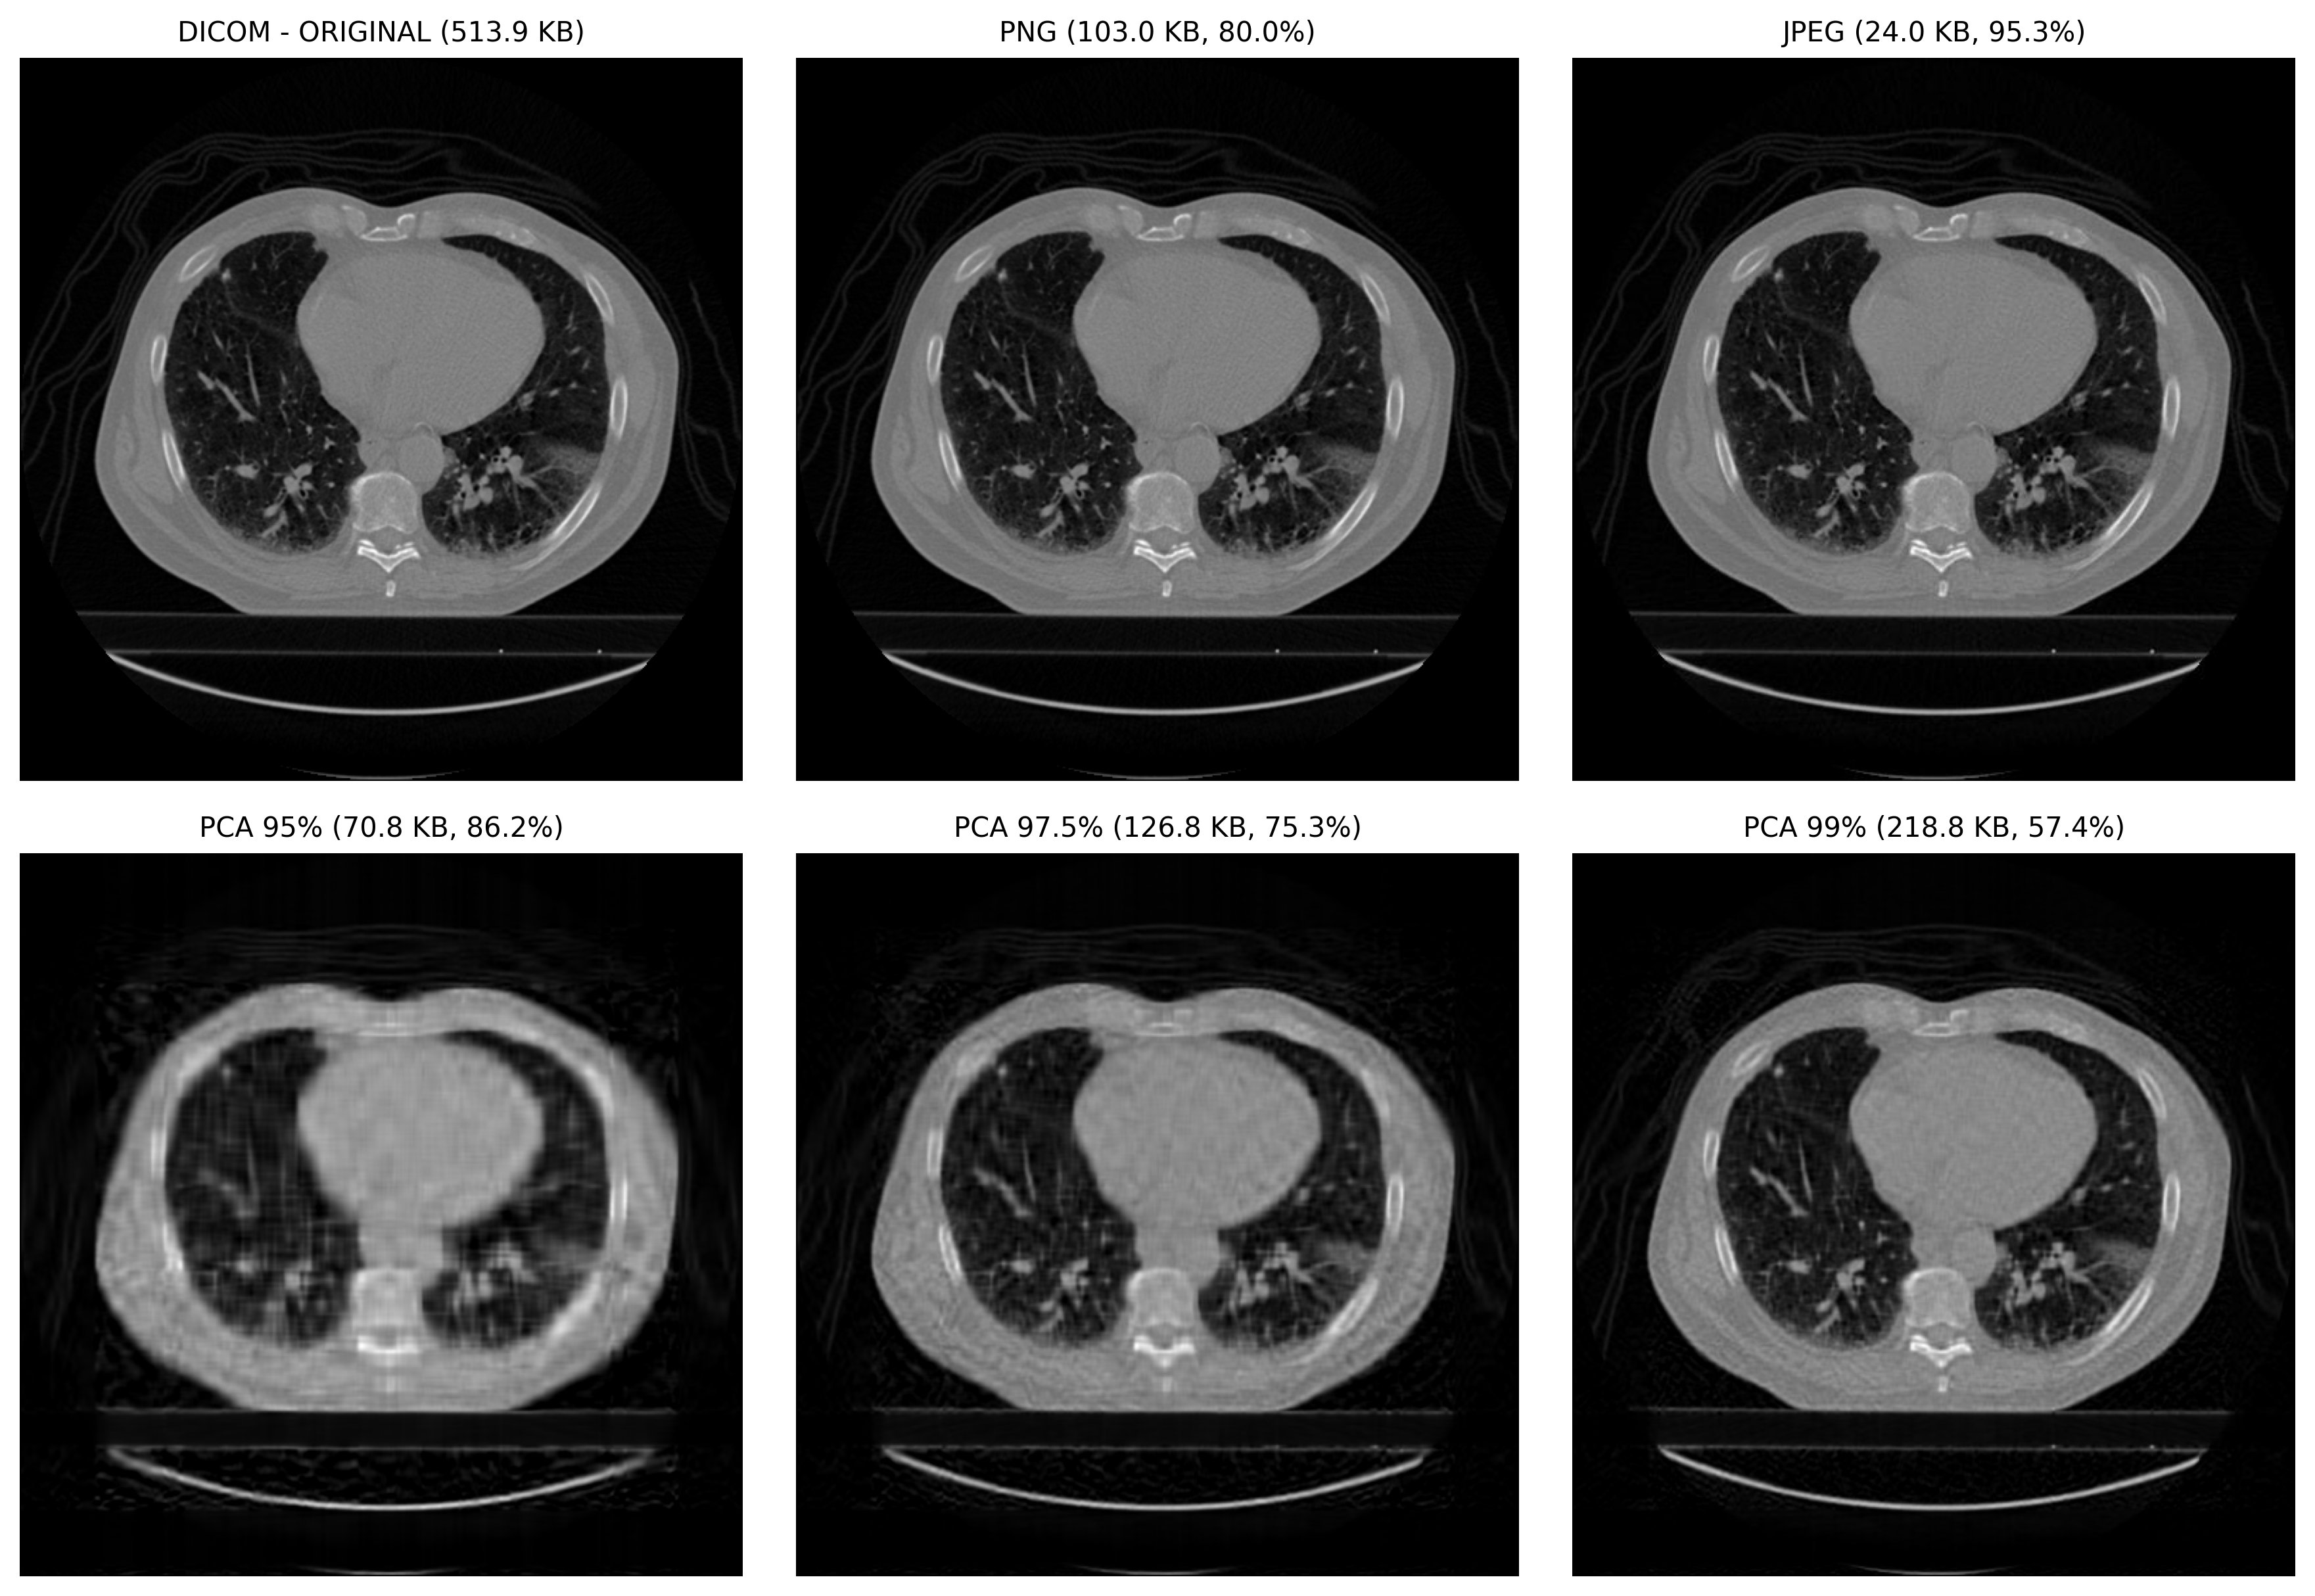
\includegraphics[width=\textwidth]{images/result-lung.png}
        }{
            \Fonte{Elaborado pelo autor.}
        }	
    \end{figure}
    \item \textbf{Mama:} A Figura~\ref{fig:comparacao_mama} apresenta as imagens de mama, que possuem alta densidade de detalhes. Essa característica dificultou a compressão, especialmente em cenários de maior redução, como o \acrshort{PCA} em 95\%, resultando em perdas mais perceptíveis visualmente.
    \begin{figure}[H]
        \centering
        \UNIFORfig{
            \Caption{\label{fig:comparacao_mama} Comparação visual das imagens de mama: original e comprimidas por \acrshort{PNG}, \acrshort{JPEG} e \acrshort{PCA}.}
        }{
            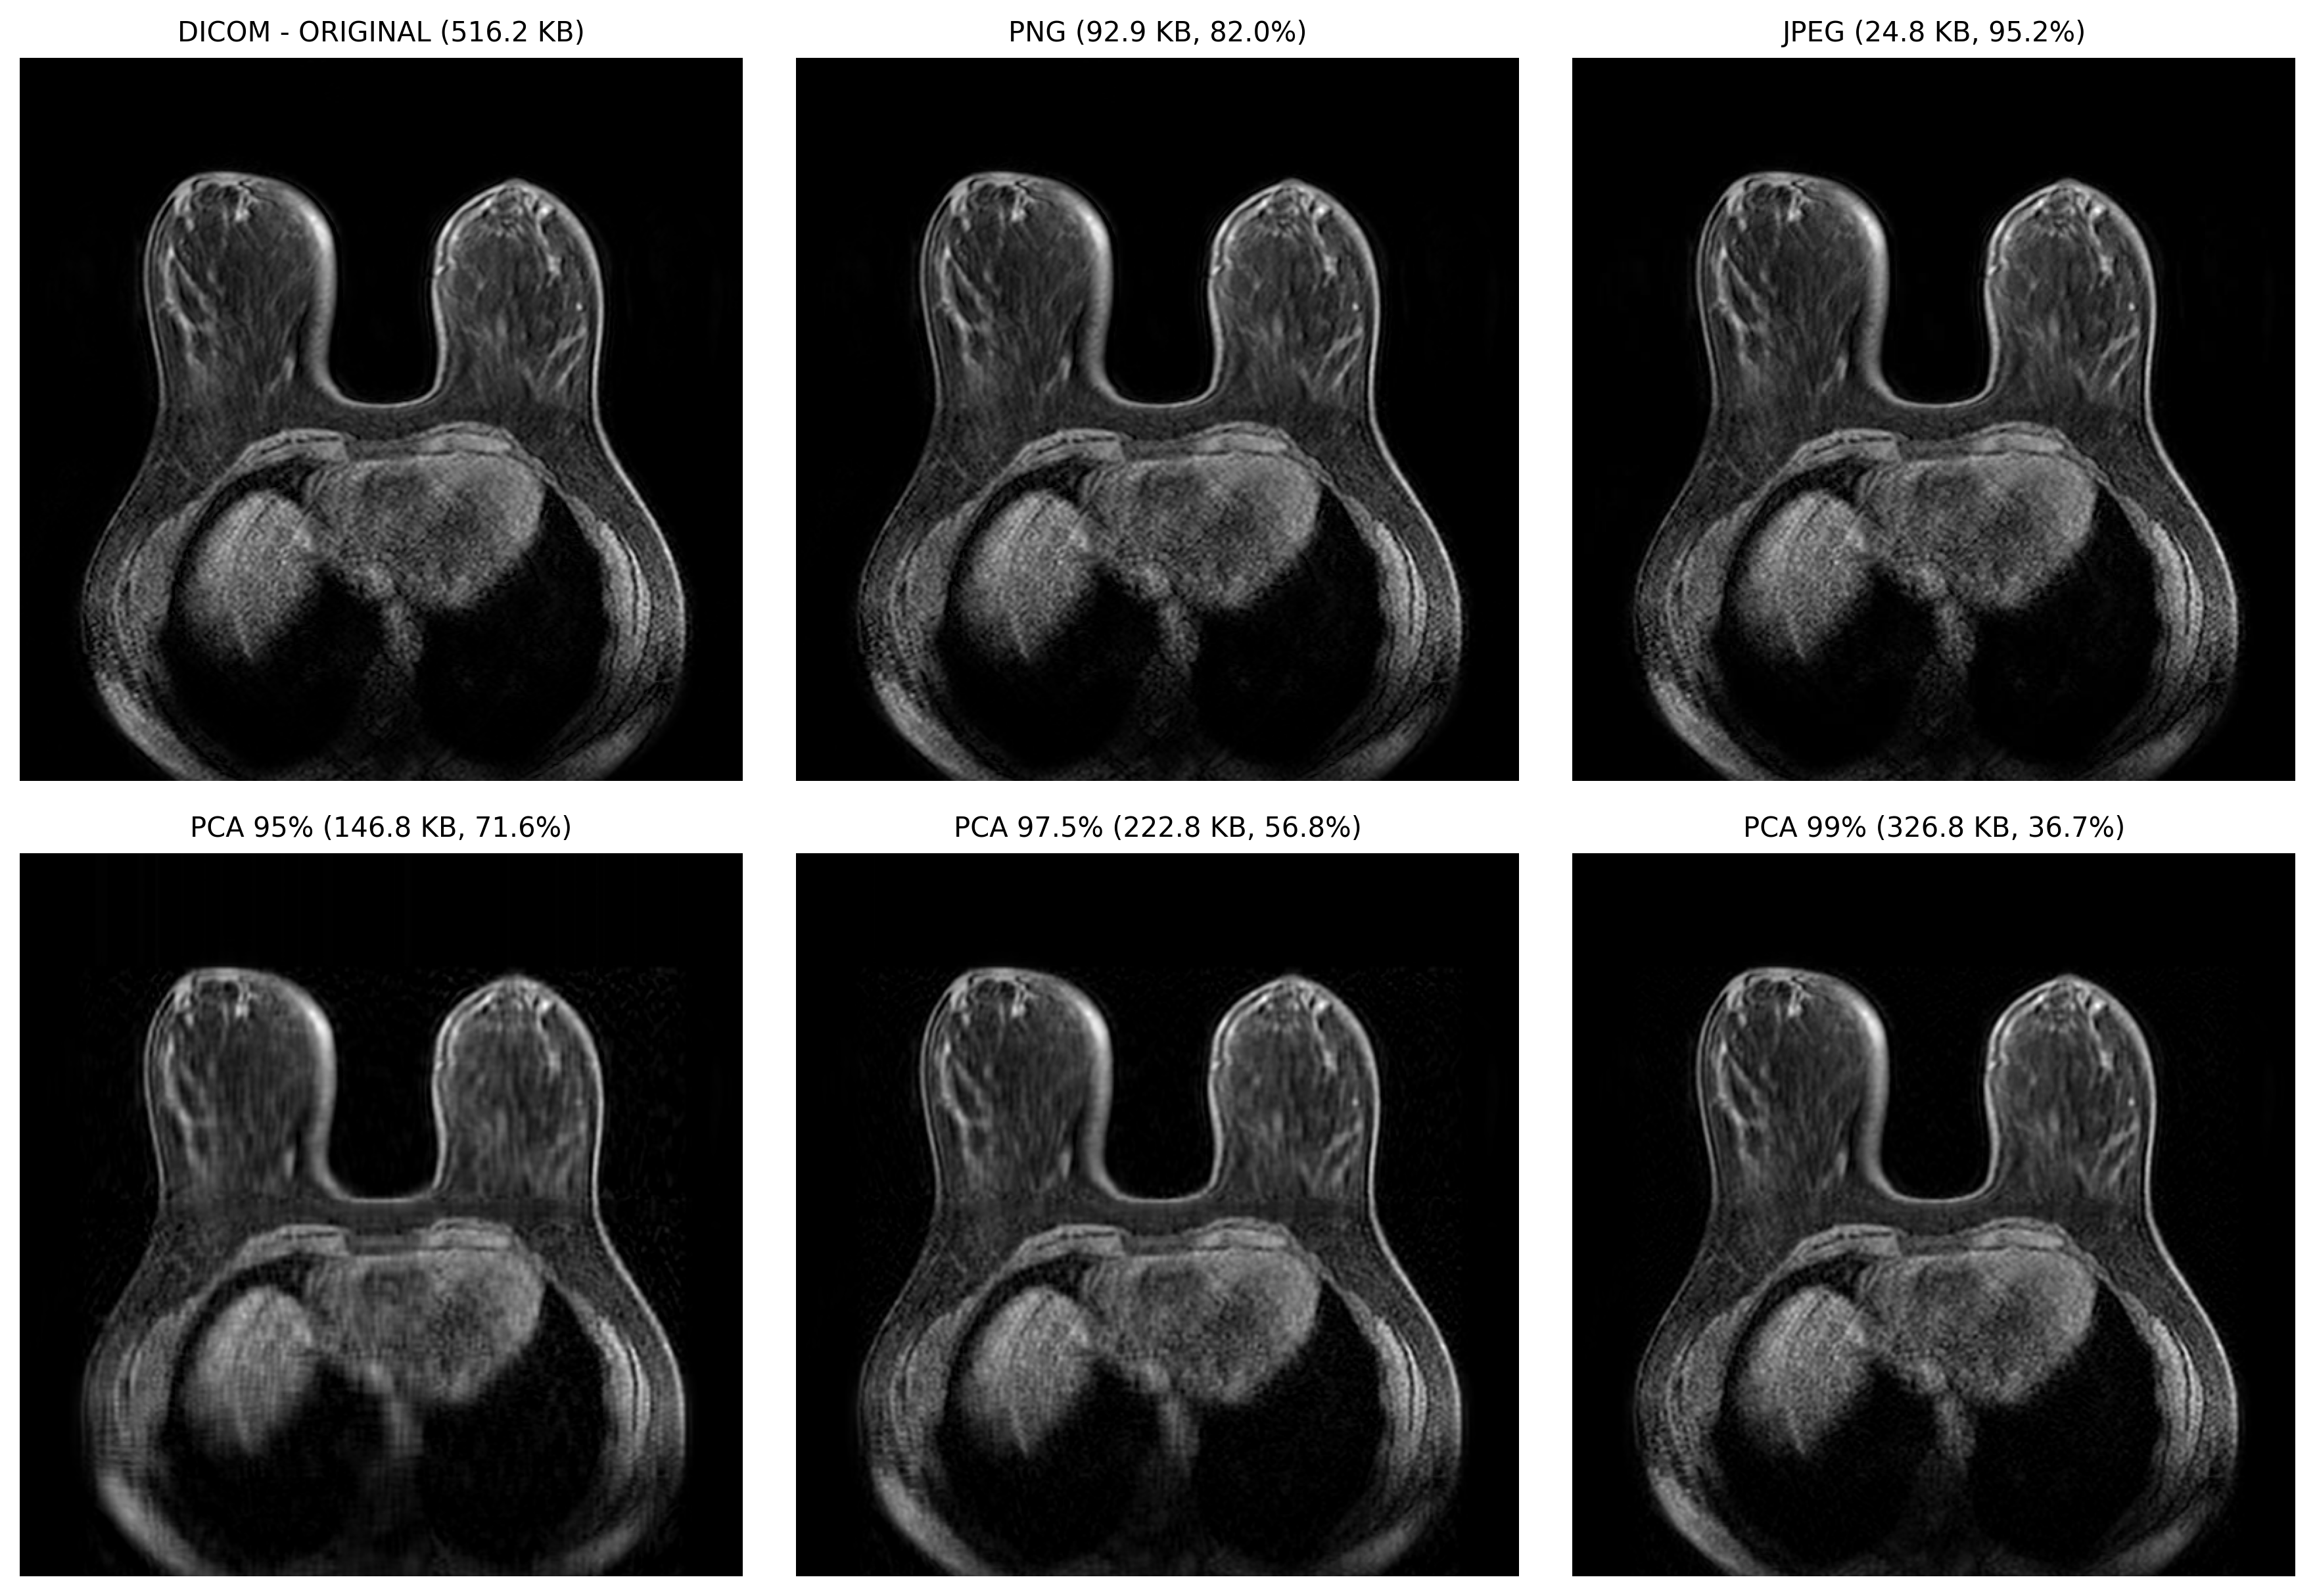
\includegraphics[width=\textwidth]{images/result-breast.png}
        }{
            \Fonte{Elaborado pelo autor.}
        }	
    \end{figure}
    \item \textbf{Cérebro:} Na Figura~\ref{fig:comparacao_cerebro}, observa-se as imagens de cérebro, que possuem uma combinação equilibrada entre áreas homogêneas e detalhadas. Essa característica resultou em compressões intermediárias, com perdas visuais moderadas dependendo do método e dos parâmetros utilizados, como observado no \acrshort{PCA}.
    \begin{figure}[H]
        \centering
        \UNIFORfig{
            \Caption{\label{fig:comparacao_cerebro} Comparação visual das imagens de cérebro: original e comprimidas por \acrshort{PNG}, \acrshort{JPEG} e \acrshort{PCA}.}
        }{
            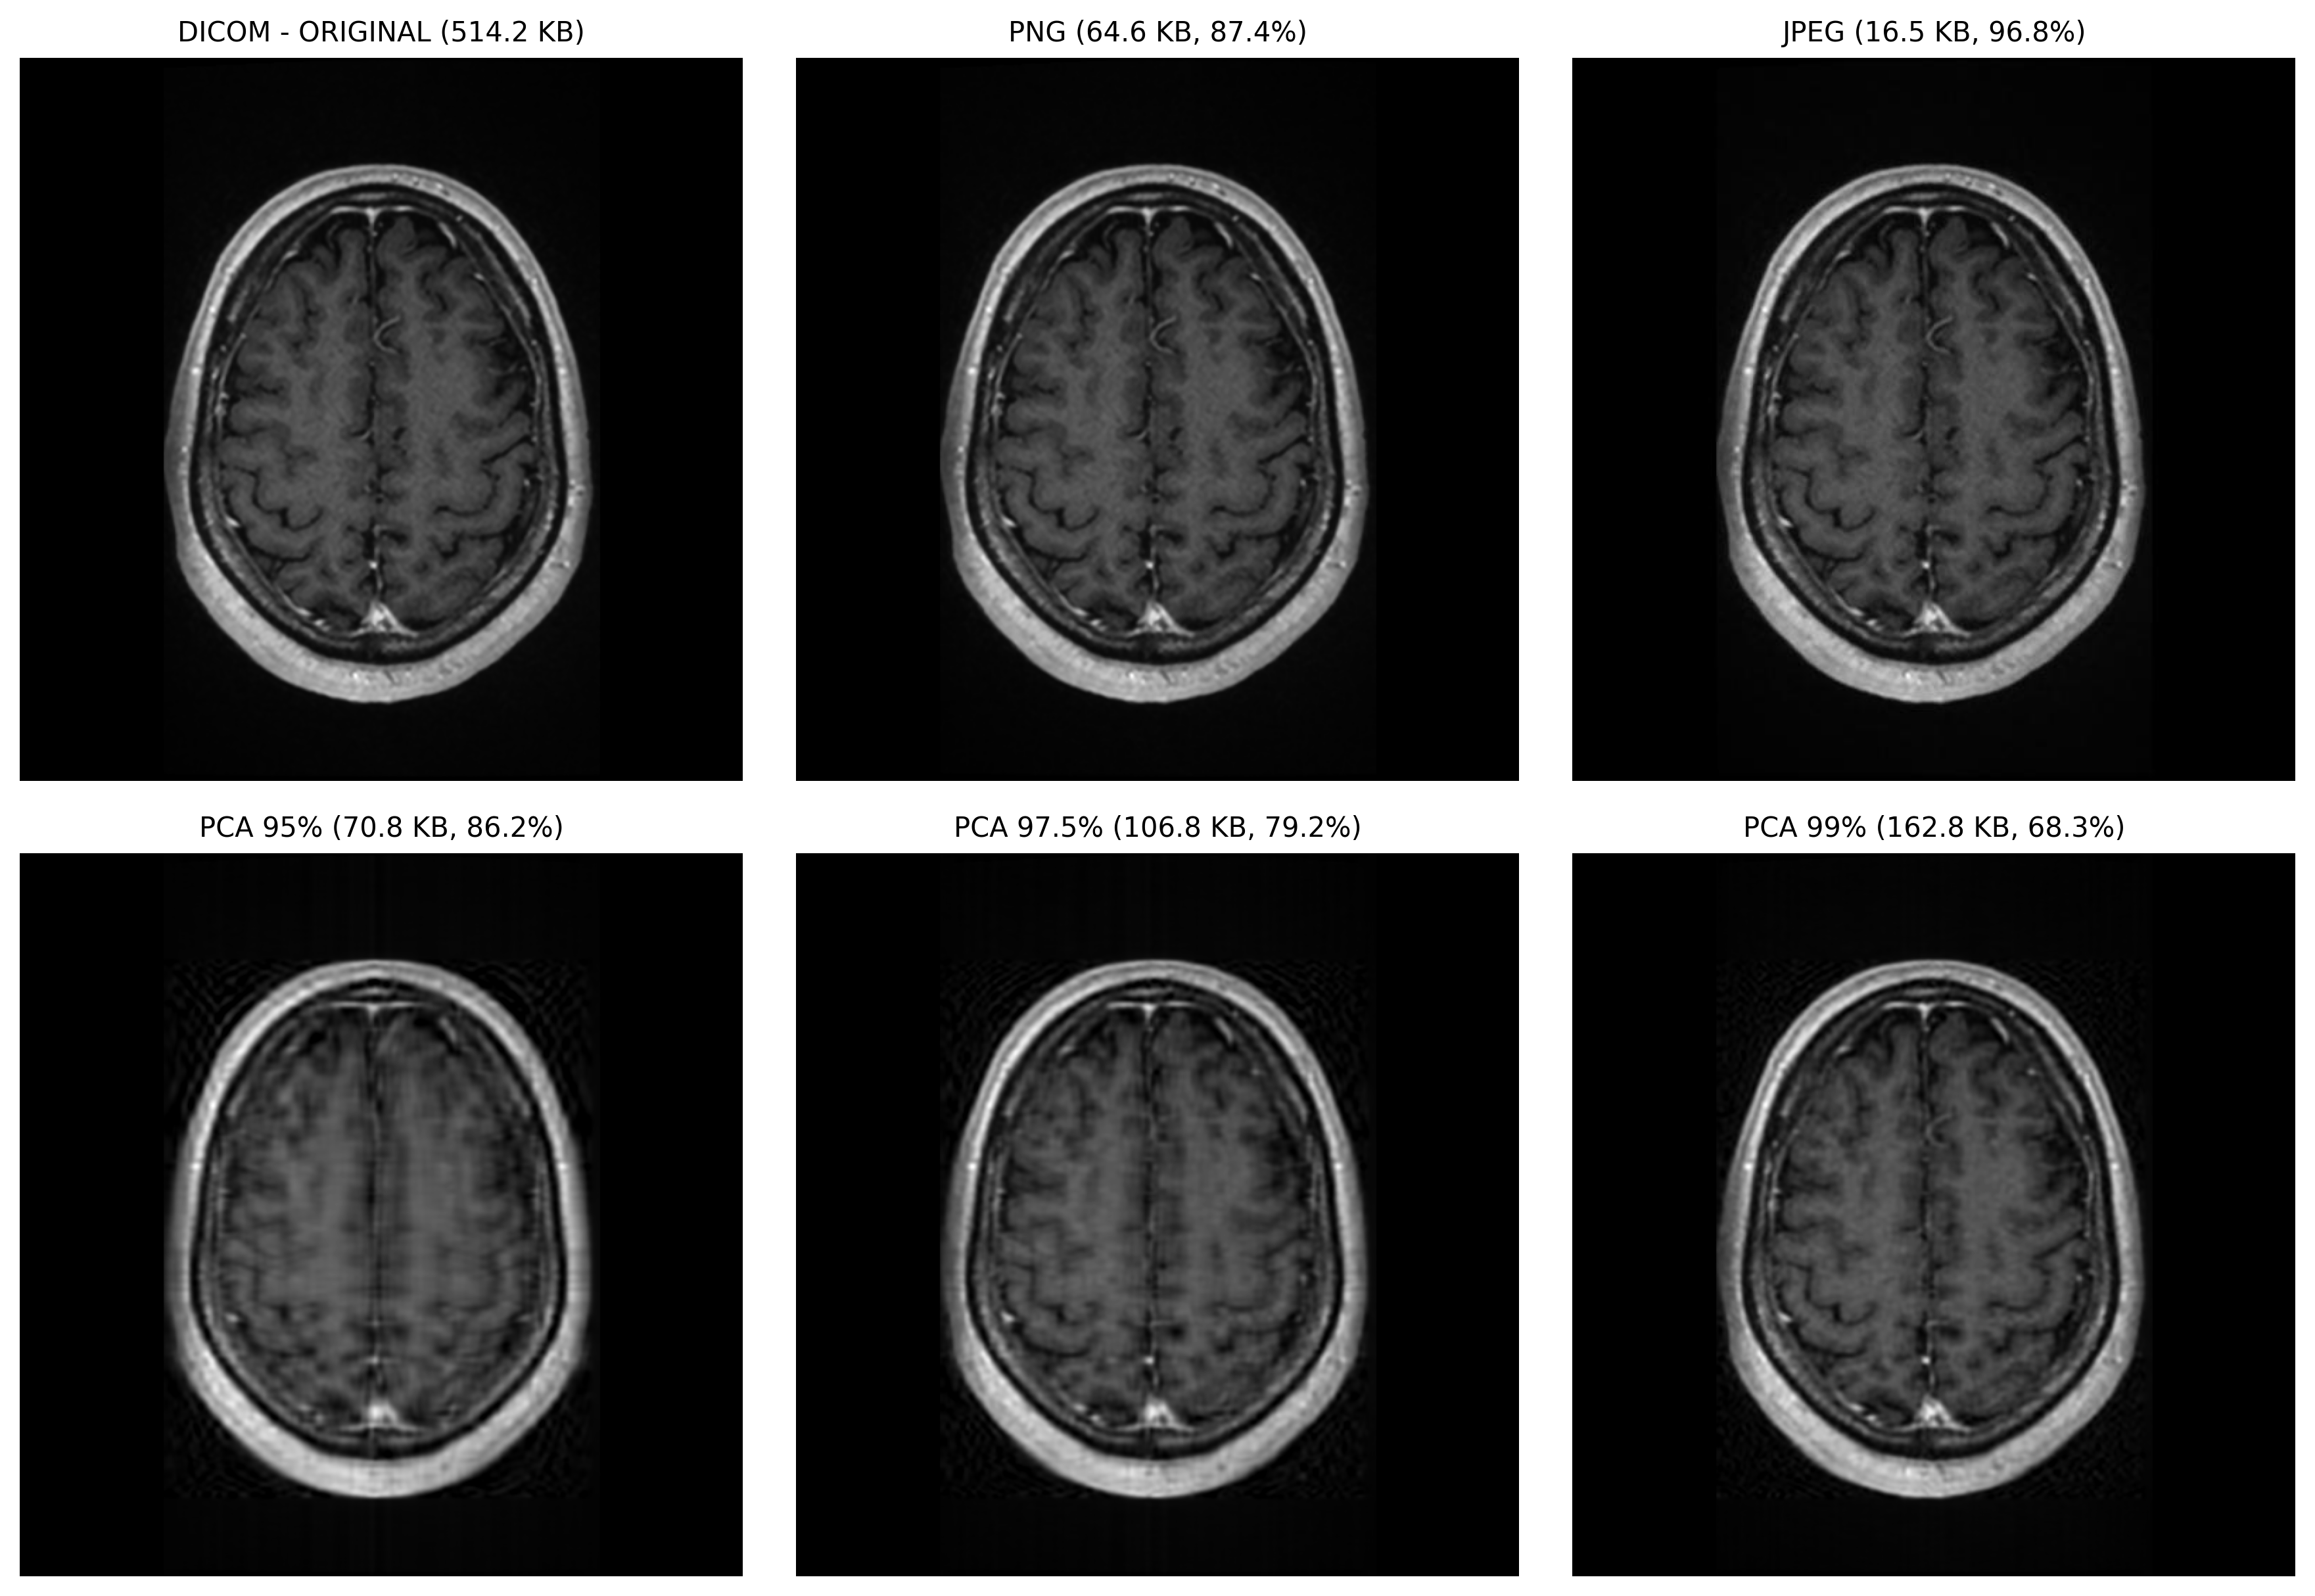
\includegraphics[width=\textwidth]{images/result-brain.png}
        }{
            \Fonte{Elaborado pelo autor.}
        }	
    \end{figure}
\end{itemize}

Estas figuras destacam que o método \acrshort{PNG} é ideal para preservação completa de qualidade, enquanto o \acrshort{JPEG} e o \acrshort{PCA} oferecem maior flexibilidade entre compressão e qualidade visual, dependendo dos parâmetros utilizados.

\section{Taxas de Compressão}

As taxas médias de compressão obtidas por cada algoritmo, agrupadas por tipo de órgão, estão apresentadas na Figura~\ref{fig:compression_by_algorithm_and_organ}. Observa-se que:

\begin{itemize}
    \item O algoritmo \textbf{\acrshort{JPEG}} alcançou as maiores taxas de compressão em todos os órgãos, superando 96\%.
    \item O \textbf{\acrshort{PNG}}, embora sem perdas, apresentou taxas de compressão em torno de 83-86\%, destacando-se pela capacidade de obter uma alta taxa de compressão mesmo sem ter perdas de informações.
    \item O \textbf{\acrshort{PCA}} teve desempenho variável conforme o percentual de variância explicada. À medida que a variância aumenta (de 95\% para 99\%), a taxa de compressão diminui, o que é esperado devido ao aumento na retenção de detalhes.
\end{itemize}

\begin{figure}[!htbp]
	\centering
	\UNIFORfig{
	    \Caption{\label{fig:compression_by_algorithm_and_organ} Taxas médias de compressão por tipo de órgão e método de compressão.}
	}{
	    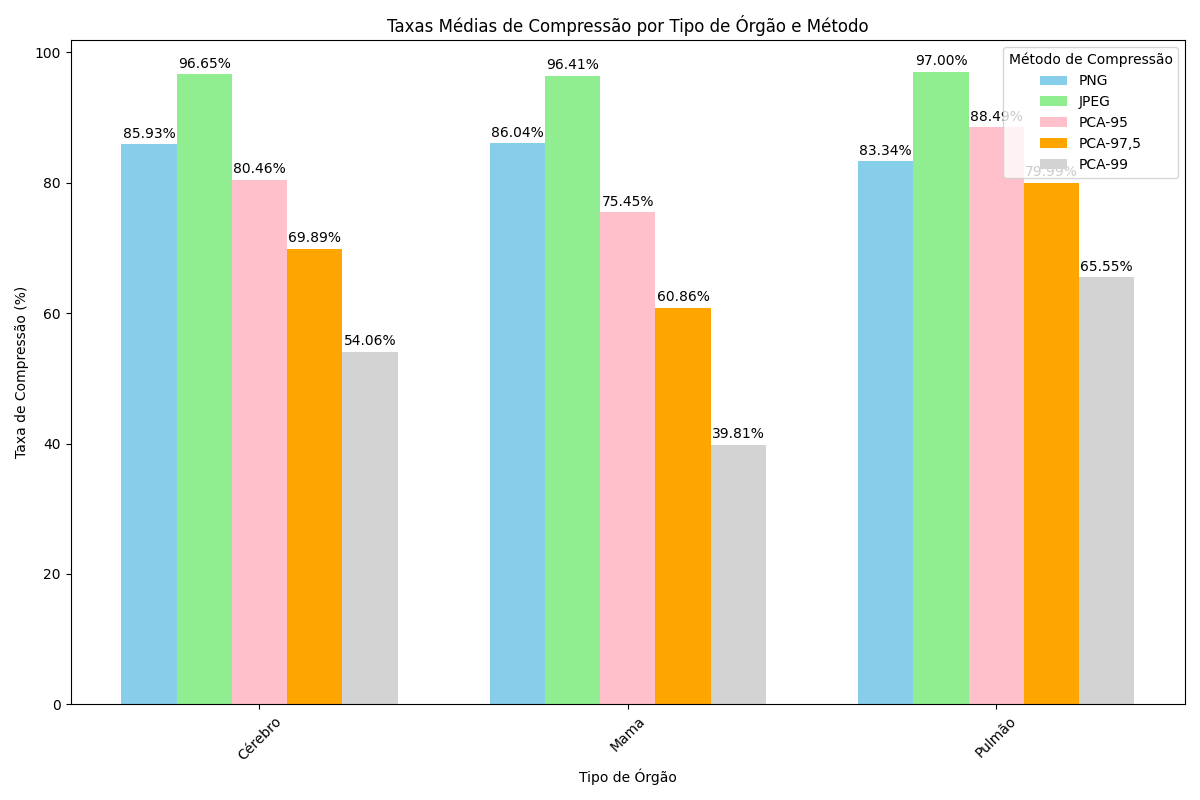
\includegraphics[width=\textwidth]{images/compression_by_algorithm_and_organ.png}
	}{
	    \Fonte{Elaborado pelo autor}
	}	
\end{figure}

\section{Taxas de Compressão por Método}

Para uma análise detalhada por algoritmo, foram gerados gráficos específicos para cada método, conforme apresentado a seguir:

\subsection{\acrshort{PNG}}

As taxas médias de compressão do \acrshort{PNG} estão ilustradas na Figura~\ref{fig:png_compression_by_organ}. O desempenho foi uniforme entre os órgãos, com taxas variando entre 83\% e 86\%.

\begin{figure}[H]
	\centering
	\UNIFORfig{
	    \Caption{\label{fig:png_compression_by_organ} Taxas médias de compressão \acrshort{PNG} por tipo de órgão.}
	}{
	    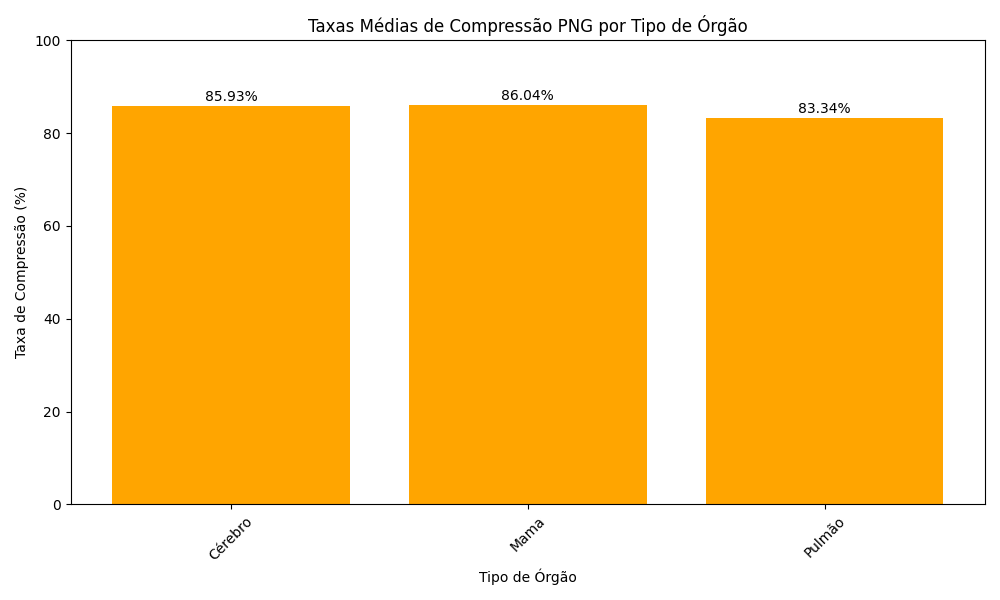
\includegraphics[width=0.8\textwidth]{images/png_compression_by_organ.png}
	}{
	    \Fonte{Elaborado pelo autor}
	}	
\end{figure}

\subsection{\acrshort{JPEG}}

A Figura~\ref{fig:jpeg_compression_by_organ} apresenta as taxas médias de compressão para o \acrshort{JPEG}. Este método apresentou as melhores taxas de compressão entre quase todos os algoritmos, alcançando valores superiores a 97\%.

\begin{figure}[H]
	\centering
	\UNIFORfig{
	    \Caption{\label{fig:jpeg_compression_by_organ} Taxas médias de compressão \acrshort{JPEG} por tipo de órgão.}
	}{
	    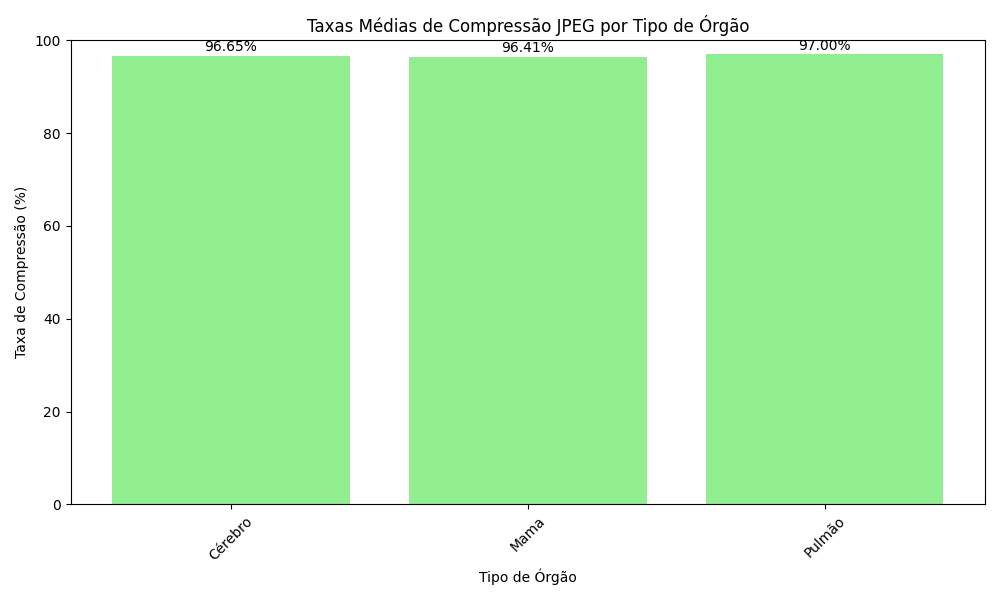
\includegraphics[width=0.8\textwidth]{images/jpeg_compression_by_organ.png}
	}{
	    \Fonte{Elaborado pelo autor}
	}	
\end{figure}

\subsection{\acrshort{PCA}}

As taxas médias de compressão para o \acrshort{PCA} são apresentadas nas Figuras~\ref{fig:pca-950}, \ref{fig:pca-975} e \ref{fig:pca-990}, referentes aos percentuais de variância explicada de 95\%, 97,5\% e 99\%, respectivamente. Observa-se que:

\begin{itemize}
    \item A compressão diminui à medida que aumenta o percentual de variância explicada, devido à retenção de mais detalhes.
    \item Órgãos com maior densidade de pixels (como pulmão) apresentam maior compressão, pois possuem mais áreas uniformes que facilitam a aplicação do \acrshort{PCA}.
\end{itemize}

\begin{figure}[H]
	\centering
	\UNIFORfig{
	    \Caption{\label{fig:pca-950} Taxas médias de compressão por tipo de órgão para o \acrshort{PCA} (95\% de variância explicada).}
	}{
	    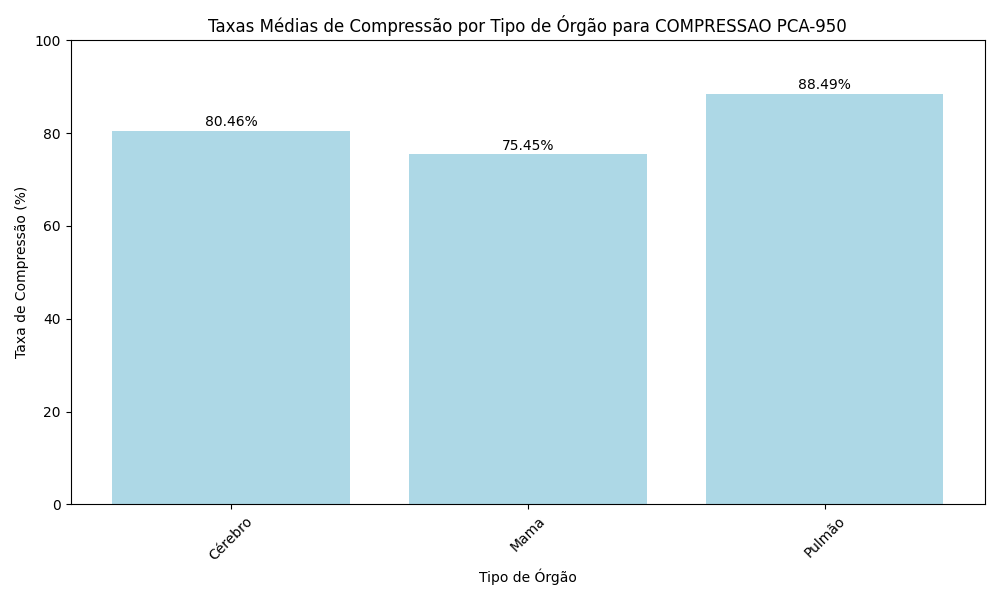
\includegraphics[width=0.8\textwidth]{images/pca-950_compression_by_organ.png}
	}{
	    \Fonte{Elaborado pelo autor}
	}	
\end{figure}

\begin{figure}[H]
	\centering
	\UNIFORfig{
	    \Caption{\label{fig:pca-975} Taxas médias de compressão por tipo de órgão para o \acrshort{PCA} (97,5\% de variância explicada).}
	}{
	    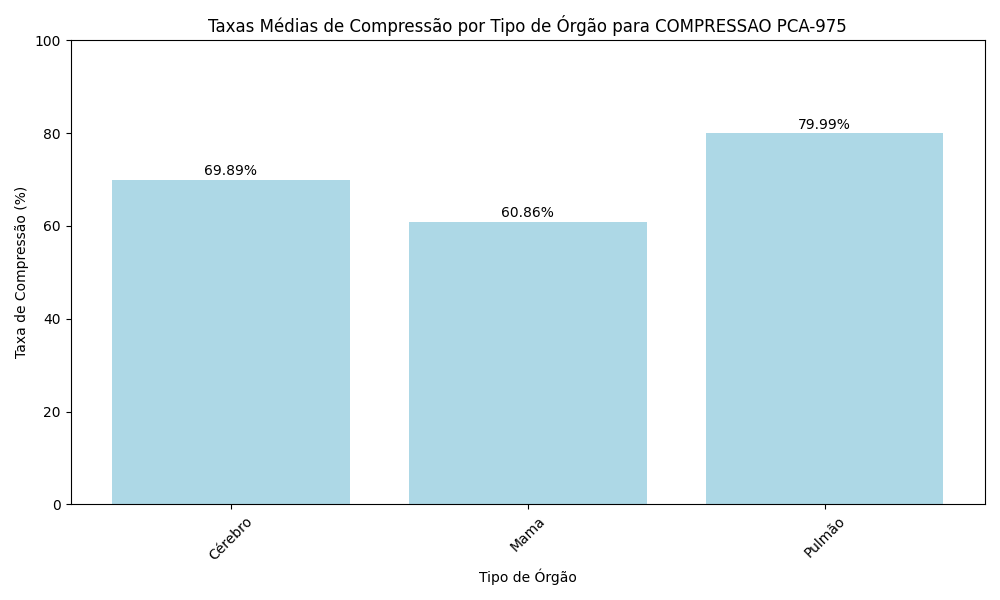
\includegraphics[width=0.8\textwidth]{images/pca-975_compression_by_organ.png}
	}{
	    \Fonte{Elaborado pelo autor}
	}	
\end{figure}

\begin{figure}[H]
	\centering
	\UNIFORfig{
	    \Caption{\label{fig:pca-990} Taxas médias de compressão por tipo de órgão para o \acrshort{PCA} (99\% de variância explicada).}
	}{
	    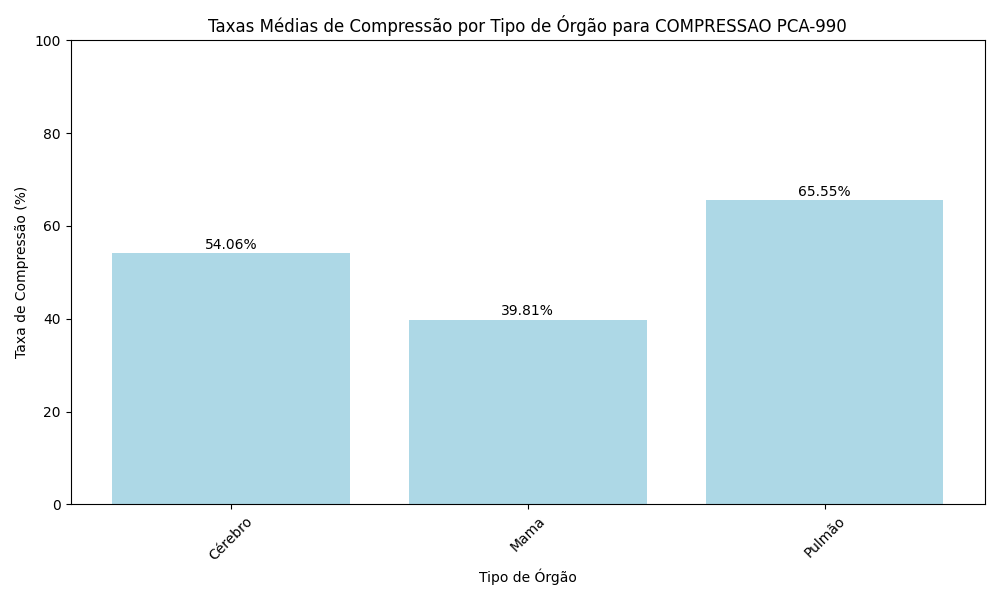
\includegraphics[width=0.8\textwidth]{images/pca-990_compression_by_organ.png}
	}{
	    \Fonte{Elaborado pelo autor}
	}	
\end{figure}

\section{Análise de Qualidade Aparente (\acrshort{PSNR})}

Os valores médios de \acrshort{PSNR} obtidos estão apresentados na Figura~\ref{fig:psnr_by_algorithm_and_organ}. Observa-se que:

\begin{itemize}
    \item O \textbf{\acrshort{PNG}} apresentou valores que tendem ao infinito, uma vez que é um método sem perda logo o \acrshort{MSE} resulta em 0, indicando qualidade visual idêntica à imagem original.
    \item O \textbf{\acrshort{JPEG}} manteve valores entre 42 e 45 dB, indicando uma alta qualidade, embora com perdas.
    \item O \textbf{\acrshort{PCA}} apresentou valores mais baixos para os percentuais de variância explicada de 95\% e 97,5\%, enquanto o PCA-99\% manteve valores próximos a 40 dB, destacando-se pela retenção de maior qualidade visual.
\end{itemize}

\begin{figure}[!htbp]
	\centering
	\UNIFORfig{
	    \Caption{\label{fig:psnr_by_algorithm_and_organ} Valores médios de \acrshort{PSNR} por algoritmo e tipo de órgão.}
	}{
	    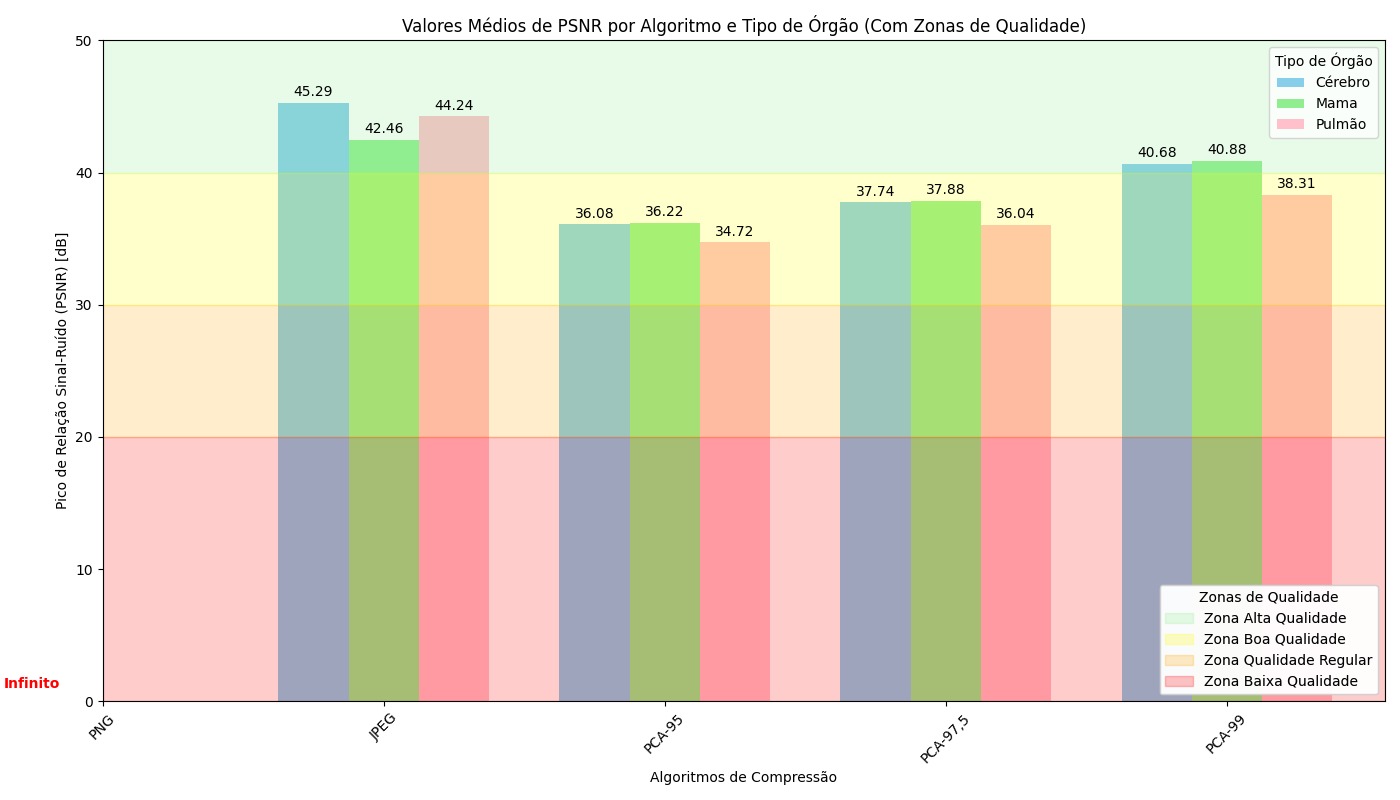
\includegraphics[width=\textwidth]{images/psnr_by_algorithm_and_organ.png}
	}{
	    \Fonte{Elaborado pelo autor}
	}	
\end{figure}

\section{Discussão dos Resultados}

Os resultados obtidos indicam que a escolha do algoritmo de compressão depende do objetivo:

\begin{itemize}
    \item O \textbf{\acrshort{PNG}} preserva integralmente a qualidade visual da imagem original, sendo indicado para casos onde a preservação completa da qualidade é imprescindível, como em aplicações críticas para diagnóstico médico. Este resultado é esperado, dado que o \acrshort{PNG} é um método de compressão sem perda, apresentando taxas de compressão consistentes e eficiência em manter a integridade das informações.
    \item O \textbf{\acrshort{JPEG}} é ideal para maximizar a compressão, mesmo com uma pequena perda de qualidade visual. Este método apresenta pequenas perdas de detalhes em áreas com maior densidade de informação (ex.: bordas e transições), mas as diferenças visuais são mínimas, tornando-o adequado para armazenamento de longo prazo e situações onde a redução significativa de tamanho é prioritária. 
    \item O \textbf{\acrshort{PCA}} oferece flexibilidade, permitindo ajustar o nível de compressão com base na variância explicada. No entanto, as diferenças visuais aumentam conforme o nível de variância explicada diminui, sendo que imagens comprimidas com 95\% de variância apresentam degradação visível em áreas de maior contraste. Em contrapartida, versões com 99\% de variância preservam melhor os detalhes visuais, ainda que com menor taxa de compressão. Esse método também requer maior processamento para reconstruir as imagens, o que deve ser considerado em contextos práticos.
\end{itemize}

A variação entre os órgãos pode ser atribuída às características específicas das imagens:

\begin{itemize}
    \item O \textbf{pulmão}, caracterizado por grandes áreas homogêneas devido à presença de espaços vazios (pretos) nas imagens de tomografia, favoreceu a compressão eficiente em todos os algoritmos. Essa característica reduz a complexidade da imagem, permitindo que métodos como o \acrshort{PCA} e o \acrshort{JPEG} explorem a redundância dos dados para alcançar altas taxas de compressão sem comprometer significativamente a qualidade visual.
    \item A \textbf{mama}, devido à sua alta densidade de detalhes e à textura mais heterogênea distribuída por toda a imagem, apresentou maior dificuldade para compressão. Essa complexidade aumenta a quantidade de informação que precisa ser mantida, especialmente para métodos como o \acrshort{PCA}, que depende de uma separação clara entre componentes principais e ruído. Como resultado, as taxas de compressão foram menores e as perdas de qualidade mais perceptíveis.
    \item O \textbf{cérebro}, com características intermediárias, combina áreas homogêneas, como o fundo da imagem, com regiões mais detalhadas, como o córtex cerebral. Essa composição balanceada permitiu que os algoritmos alcançassem resultados intermediários tanto em taxas de compressão quanto em qualidade visual. Enquanto o fundo homogêneo facilita a compressão, as regiões detalhadas impõem desafios que moderam o desempenho global dos algoritmos.
\end{itemize}

Esses resultados contribuem para a definição de estratégias eficientes de compressão em ambientes hospitalares, levando em consideração as características específicas das imagens médicas de cada órgão.

	% \chapter{Conclusão}
\label{cap:conclusao}

Neste trabalho, foi realizada uma análise comparativa de três métodos de compressão de imagens médicas no formato \acrshort{DICOM}: \acrshort{PNG}, \acrshort{JPEG} e \acrshort{PCA}. O estudo investigou o impacto desses algoritmos na redução do tamanho dos arquivos e na preservação da qualidade das imagens médicas, considerando três tipos de órgãos: pulmão, mama e cérebro. Os resultados demonstraram diferenças significativas entre os métodos, evidenciando vantagens e limitações que dependem tanto das características dos algoritmos quanto do conteúdo das imagens.

As questões de pesquisa levantadas foram abordadas de maneira detalhada. Primeiramente, quanto às taxas médias de compressão alcançadas pelos algoritmos, o \acrshort{JPEG} obteve os melhores resultados, superando 96\% em todos os órgãos analisados. O \acrshort{PNG} apresentou taxas moderadas e consistentes de 83-86\%, conciliando uma alta taxa de compressão com preservação total da qualidade. Já o \acrshort{PCA} demonstrou um desempenho variável, dependendo do percentual de variância explicada, sendo mais eficiente em cenários onde a retenção parcial da informação é aceitável.

Sobre o impacto das características das imagens de cada órgão nas taxas de compressão, foi constatado que imagens de pulmão, devido às suas grandes áreas homogêneas, favoreceram a compressão em todos os algoritmos, resultando nas melhores taxas. Por outro lado, as imagens de mama, com maior densidade de detalhes, apresentaram maior resistência à compressão. As imagens de cérebro, por sua vez, exibiram comportamento intermediário, refletindo sua composição equilibrada entre áreas homogêneas e detalhadas.

Em relação ao impacto da variação da taxa de compressão na qualidade visual, os valores de \acrshort{PSNR} demonstraram que o \acrshort{PNG} manteve a qualidade perfeita das imagens, com \acrshort{PSNR} tendendo ao infinito. O \acrshort{JPEG} apresentou valores entre 42 e 45 dB, indicando alta qualidade visual com perdas imperceptíveis a olho nu. Já o \acrshort{PCA}, dependendo do percentual de variância explicada, teve qualidade mais variável, com melhores resultados observados em níveis mais altos (99\%).

Finalmente, no que diz respeito à escolha do algoritmo ideal para cada cenário, conclui-se que o \acrshort{JPEG} oferece o melhor equilíbrio entre compressão e qualidade visual, sendo uma opção eficiente para armazenamento em larga escala. O \acrshort{PNG} é recomendado para aplicações que exigem preservação total da qualidade, enquanto o \acrshort{PCA} é mais indicado para cenários onde a flexibilidade na retenção de dados é prioritária, apesar de seu maior custo computacional.

Este estudo contribui para o entendimento das particularidades de cada método de compressão e oferece subsídios para a escolha de estratégias adequadas em diferentes cenários hospitalares. Como trabalhos futuros, sugere-se:
\begin{itemize}
    \item Avaliar outros algoritmos de compressão, como \acrshort{AVIF} e \acrshort{SPIHT}, que também são amplamente utilizados em imagens médicas e científicas.
    \item Explorar métodos baseados em aprendizado de máquina, como compressão neural.
    \item Investigar o impacto da compressão na acurácia de diagnósticos realizados a partir dessas imagens com o auxílio de um profissional da saúde especializado em diagnóstico de imagens médicas.
    \item Ampliar o estudo para outros tipos de exames médicos, como ressonância magnética e ultrassonografia, a fim de verificar se os resultados observados neste trabalho se mantêm em outros contextos.
\end{itemize}

Com base nos resultados obtidos, conclui-se que a compressão de imagens médicas, quando bem planejada, pode oferecer soluções eficazes para os desafios de armazenamento em ambientes hospitalares, conciliando redução de tamanho e preservação da integridade das informações essenciais ao diagnóstico.



	%Elementos pós-textuais
	\bibliography{elementos-pos-textuais/referencias}
	%\imprimirglossario
    % \imprimirapendices
	% Adicione aqui os apendices do seu trabalho
		% \input{elementos-pos-textuais/apendices/Algoritmo}
		% % \apendice{Entradas passageiros}
% \label{ap:Entradas}
		% % \apendice{Entradas voos}
% \label{ap:EntradaVoos}

		% % \apendice{Resultados}
% \label{ap:resultados}

%	\imprimiranexos
		% Adicione aqui os anexos do seu trabalho
%		\input{elementos-pos-textuais/anexos/exemplo-de-anexo}
%		\anexo{Dinâmica das classes sociais}
\label{an:dinamica-das-classes-sociais}

\lipsum[14]
\index{AAA}
%	\imprimirindice

\end{document}
